\documentclass[10pt]{article}
\usepackage[T1]{fontenc}
\usepackage[headheight=1.5cm,top=3cm,left=2cm,right=2cm]{geometry}
\usepackage{amsfonts}
\usepackage{helvet}
\usepackage{longtable}
\usepackage{hyperref}
\usepackage{graphicx}

\usepackage{caption}
\usepackage{subcaption}

\usepackage[dvipsnames]{xcolor}
\usepackage{float}
\usepackage{fancyhdr}
\usepackage{multirow}
\usepackage{array}
\newcolumntype{L}[1]{>{\raggedright\let\newline\\\arraybackslash\hspace{0pt}}m{#1}}
\newcolumntype{C}[1]{>{\centering\let\newline\\\arraybackslash\hspace{0pt}}m{#1}}
\newcolumntype{R}[1]{>{\raggedleft\let\newline\\\arraybackslash\hspace{0pt}}m{#1}}


\usepackage{stackengine}
\newcommand\No[1][.13ex]{%
  \setbox0=\hbox{\scalebox{.7}{o}}%
  \setbox2=\hbox{N}%
  N\kern-.05em\stackengine{\dimexpr\ht0-\ht2+#1}{\belowbaseline[-\ht2]{\copy0}}%
    {\rule[-.13ex]{.7\wd0}{.13ex}}%
    {U}{c}{F}{F}{L}%
}


\usepackage{pbox}
\usepackage{pgf,tikz,pgfplots}
\pgfplotsset{compat=1.15}
\usepackage{mathrsfs}
\usetikzlibrary{arrows}
\definecolor{qqqqff}{rgb}{0,0,1}
\definecolor{ffqqqq}{rgb}{1,0,0}

\usepackage{color, colortbl}
\usetikzlibrary{arrows,positioning}
\renewcommand{\familydefault}{\sfdefault}
\setlength{\parindent}{0pt}
\setlength{\parskip}{10pt}
\pagestyle{fancy}
\renewcommand{\headrulewidth}{0.0pt}
\fancyhf{}

\newcommand{\doctitle}{MNIST Training}
\newcommand{\docauthor}{Document Author}

\title{\doctitle}
\author{\docauthor}

\renewcommand{\labelenumii}{\theenumii}
\renewcommand{\theenumii}{\theenumi.\arabic{enumii}.}
\usepackage{enumitem}

\usepackage{listings}

\newcommand{\dev}[1]{{\sc #1}}

\usepackage{siunitx}
\usepackage{tabularx}
\newcolumntype{L}[1]{>{\raggedright\arraybackslash}p{#1}}
\newcolumntype{C}[1]{>{\centering\arraybackslash}p{#1}}
\newcolumntype{R}[1]{>{\raggedleft\arraybackslash}p{#1}}


\definecolor{InputLayer}{RGB}{44, 189, 201} %light blue

\definecolor{Conv2D}{RGB}{235, 101, 52} % orange/red
\definecolor{Dense}{RGB}{235, 52, 55} %red
\definecolor{BatchNormalization}{RGB}{235, 52, 140} %pink

\definecolor{Activation}{RGB}{92, 52, 235} %blue
\definecolor{Dropout}{RGB}{50, 81, 168} %blue
\definecolor{MaxPooling2D}{RGB}{174, 52, 235} %purple
\definecolor{UpSampling2D}{RGB}{52, 107, 235} %lighter blue

\definecolor{Flatten}{RGB}{50, 168, 70} %Green
\definecolor{Concatenate}{RGB}{81,168,50} %Green
\definecolor{Add}{RGB}{50, 168, 121} % Blueish green

\setcounter{tocdepth}{2}
\begin{document}


$\,$\\[-2ex]
\begin{flushright}
    {\huge{\bf
    \doctitle
    }}\\[1ex]
    {\large
    \docauthor
    }
\end{flushright}

\tableofcontents
% %%%%%%%%%%%%%%%%%%%%%%%%%%%%%%%%%%%%%%%%%%%%%%%%%%%%%%%%%%%%%%%%%%%
\section{Summary}
\begin{tabular}{rrrrrrrr}
    \hline\\[-1.5ex]
    \No{} & Model name & \#Parameters & \#Epochs & Batch size & Test Acc. & Training Acc. \\
    \hline\\[-1.5ex]

    \hyperref[training:1]
             {1} &
    \hyperref[model:ConvNet2layers]
             {ConvNet2layers} &
    \num{1199882} &
    5
    &
    128 &
    98.94 \% &
    98.71 \%
    \\[4pt]
    \hyperref[training:2]
             {2} &
    \hyperref[model:ConvNet2layers]
             {ConvNet2layers} &
    \num{1199882} &
    5
    &
    128 &
    99.02 \% &
    98.73 \%
    \\[4pt]
    \hyperref[training:3]
             {3} &
    \hyperref[model:ConvNet2layers]
             {ConvNet2layers} &
    \num{1199882} &
    5
    &
    128 &
    99.07 \% &
    98.66 \%
    \\[4pt]
    \hyperref[training:4]
             {4} &
    \hyperref[model:ConvNet2layers]
             {ConvNet2layers} &
    \num{1199882} &
    5
    &
    128 &
    99.06 \% &
    98.66 \%
    \\[4pt]
    \hyperref[training:5]
             {5} &
    \hyperref[model:MLP2layers]
             {MLP2layers} &
    \num{669706} &
    1
    &
    128 &
    89.83 \% &
    88.29 \%
    \\[4pt]
    \hyperref[training:6]
             {6} &
    \hyperref[model:MLP2layers]
             {MLP2layers} &
    \num{669706} &
    5
    &
    128 &
    92.72 \% &
    92.66 \%
    \\[4pt]
    \hyperref[training:7]
             {7} &
    \hyperref[model:MLP2layers]
             {MLP2layers} &
    \num{669706} &
    5
    &
    128 &
    91.21 \% &
    90.94 \%
    \\[4pt]
    \hyperref[training:8]
             {8} &
    \hyperref[model:MLP2layers]
             {MLP2layers} &
    \num{669706} &
    5
    &
    128 &
    92.62 \% &
    92.78 \%
    \\[4pt]
    \hyperref[training:9]
             {9} &
    \hyperref[model:MLP2layers]
             {MLP2layers} &
    \num{669706} &
    5
    &
    128 &
    90.79 \% &
    91.43 \%
    \\[4pt]
    \hyperref[training:10]
             {10} &
    \hyperref[model:MLP5layers]
             {MLP5layers} &
    \num{430602} &
    5
    &
    128 &
    91.93 \% &
    89.04 \%
    \\[4pt]
    \hyperref[training:11]
             {11} &
    \hyperref[model:MLP5layers]
             {MLP5layers} &
    \num{430602} &
    5
    &
    128 &
    90.34 \% &
    86.2 \%
    \\[4pt]
    \hline
\end{tabular}
% %%%%%%%%%%%%%%%%%%%%%%%%%%%%%%%%%%%%%%%%%%%%%%%%%%%%%%%%%%%%%%%%%%%
\newpage
% %%%%%%%%%%%%%%%%%%%%%%%%%%%%%%%%%%%%%%%%%%%%%%%%%%%%%%%%%%%%%%%%%%%
\section{Training reports}
    \subsection{Model 1:
                        ConvNet2layers
                \label{training:1}
                }
    %
    \paragraph*{Training history} See Figure \ref{fig:results1}.
    \begin{figure}[H]
        \centering
        \begin{subfigure}{.5\textwidth}
            % This file was created by tikzplotlib v0.8.2.
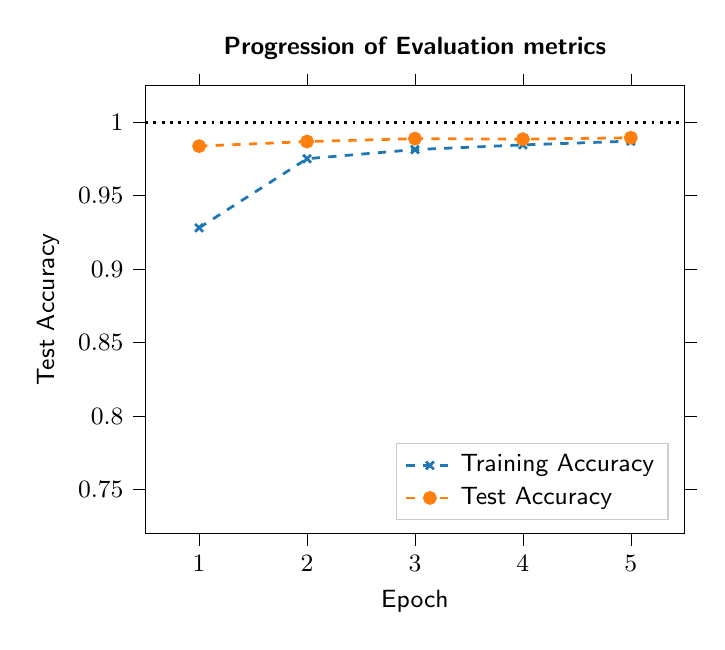
\begin{tikzpicture}

\definecolor{color0}{rgb}{0.12156862745098,0.466666666666667,0.705882352941177}
\definecolor{color1}{rgb}{1,0.498039215686275,0.0549019607843137}

\begin{axis}[
font=\small,
legend cell align={left},
legend style={at={(0.97,0.03)}, anchor=south east, draw=white!80.0!black},
minor xtick={},
minor ytick={},
tick align=outside,
tick pos=both,
title={{\bf Progression of Evaluation metrics}},
x grid style={white!69.01960784313725!black},
xlabel={Epoch},
xmin=0.5, xmax=5.5,
xtick style={color=black},
xtick={1,2,3,4,5},
y grid style={white!69.01960784313725!black},
ylabel={Test Accuracy},
ymin=0.72, ymax=1.025,
ytick style={color=black},
ytick={0.7,0.75,0.8,0.85,0.9,0.95,1,1.05}
]
\addplot [line width=1.0pt, color0, dashed, mark=x, mark size=2, mark options={solid}]
table {%
1 0.928099999968211
2 0.975133333301544
3 0.981333333301544
4 0.984533333365122
5 0.9871
};
\addlegendentry{Training Accuracy}
\addplot [line width=1.0pt, color1, dashed, mark=*, mark size=2, mark options={solid}]
table {%
1 0.9837
2 0.9868
3 0.9888
4 0.9884
5 0.9894
};
\addlegendentry{Test Accuracy}
\addplot [line width=1.0pt, black, dotted, forget plot]
table {%
0.5 1
5.5 1
};
\end{axis}

\end{tikzpicture}
            \caption{Accuracy learning process for model \protect\hyperref[training:1]
                        {1}.}
        \end{subfigure}%
        \hfill%
        \begin{subfigure}{.5\textwidth}
            % This file was created by tikzplotlib v0.8.2.
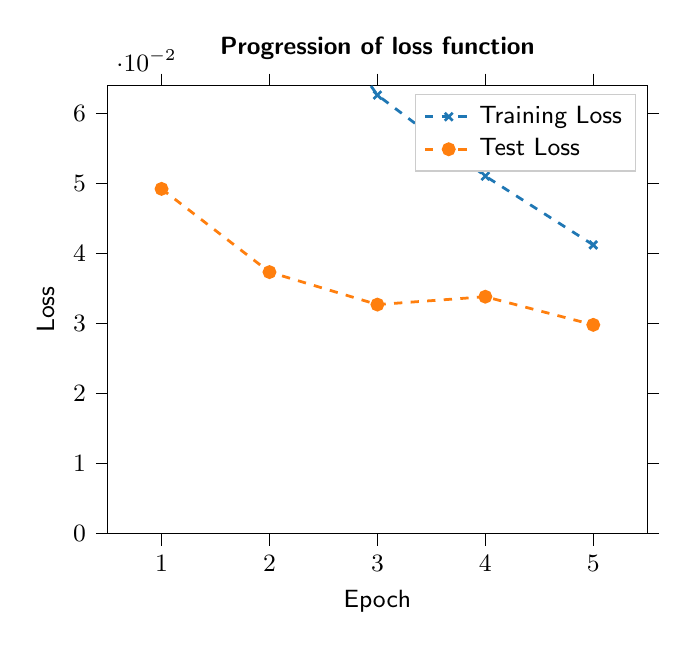
\begin{tikzpicture}

\definecolor{color0}{rgb}{0.12156862745098,0.466666666666667,0.705882352941177}
\definecolor{color1}{rgb}{1,0.498039215686275,0.0549019607843137}

\begin{axis}[
font=\small,
legend cell align={left},
legend style={draw=white!80.0!black},
minor xtick={},
minor ytick={},
tick align=outside,
tick pos=both,
title={{\bf Progression of loss function}},
x grid style={white!69.01960784313725!black},
xlabel={Epoch},
xmin=0.5, xmax=5.5,
xtick style={color=black},
xtick={1,2,3,4,5},
y grid style={white!69.01960784313725!black},
ylabel={Loss},
ymin=0, ymax=0.0640378326845914,
ytick style={color=black},
ytick={0,0.01,0.02,0.03,0.04,0.05,0.06,0.07}
]
\addplot [line width=1.0pt, color0, dashed, mark=x, mark size=2, mark options={solid}]
table {%
1 0.236453638211886
2 0.0844968503316244
3 0.0626584908445676
4 0.0510810207923253
5 0.0412529175231854
};
\addlegendentry{Training Loss}
\addplot [line width=1.0pt, color1, dashed, mark=*, mark size=2, mark options={solid}]
table {%
1 0.0492598712958396
2 0.0373745440721512
3 0.0327327600388089
4 0.0338562947141938
5 0.0298384289460373
};
\addlegendentry{Test Loss}
\end{axis}

\end{tikzpicture}
            \caption{Loss learning process for model \protect\hyperref[training:1]
                        {1}.}
        \end{subfigure}
        \par\bigskip
        \begin{subfigure}{.5\textwidth}
            % This file was created by tikzplotlib v0.8.2.
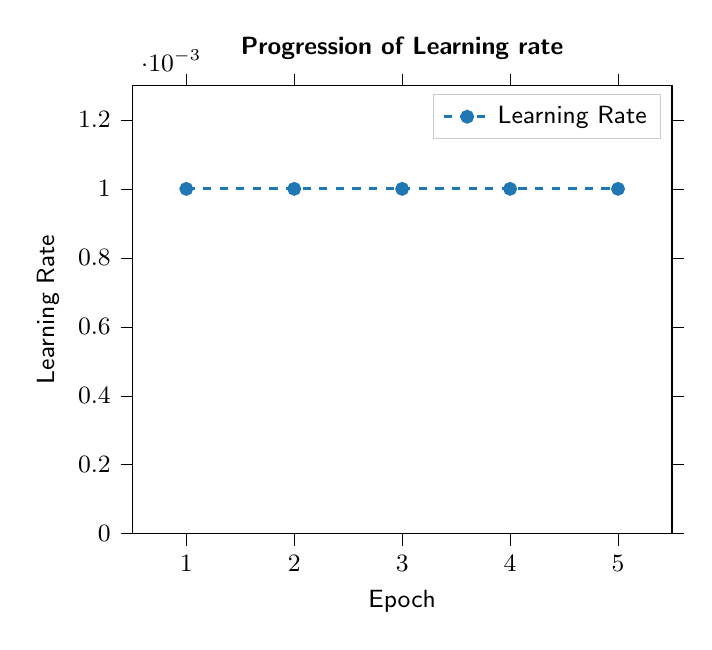
\begin{tikzpicture}

\definecolor{color0}{rgb}{0.12156862745098,0.466666666666667,0.705882352941177}

\begin{axis}[
font=\small,
legend cell align={left},
legend style={draw=white!80.0!black},
minor xtick={},
minor ytick={},
tick align=outside,
tick pos=both,
title={{\bf Progression of Learning rate}},
x grid style={white!69.01960784313725!black},
xlabel={Epoch},
xmin=0.5, xmax=5.5,
xtick style={color=black},
xtick={1,2,3,4,5},
y grid style={white!69.01960784313725!black},
ylabel={Learning Rate},
ymin=0, ymax=0.0013,
ytick style={color=black},
ytick={0,0.0002,0.0004,0.0006,0.0008,0.001,0.0012,0.0014}
]
\addplot [line width=1.0pt, color0, dashed, mark=*, mark size=2, mark options={solid}]
table {%
1 0.001
2 0.001
3 0.001
4 0.001
5 0.001
};
\addlegendentry{Learning Rate}
\end{axis}

\end{tikzpicture}
            \caption{Learning rate per epoch for model \protect\hyperref[training:1]
                        {1}.}
        \end{subfigure}%
        \caption{Training and evaluation metrics for model  \protect\hyperref[training:1]
                    {1}.
                \label{fig:results1}}
    \end{figure}

    \subsubsection*{Dataset}
    \begin{description}
        \item[Name] MNIST
        \item[Train-Test-Dev split:] {\it Training set:}
        60000,
        {\it Test set:}
        10000,
        {\it Dev set:}
        0,
        \item[Image size] [28, 28]


    \end{description}
    %
    \subsubsection*{Training}
    \begin{description}
        \item[Number of epochs] 5
        \item[Optimizer] Adam (Kingma et al., 2015)

            \begin{tabular}{rl}
                    {\bf Learning Rate} & 0.0010000000474974513 \\
                    {\bf Beta 1} & 0.8999999761581421 \\
                    {\bf Beta 2} & 0.9990000128746033 \\
                    {\bf Decay} & 0.0 \\
                    {\bf Epsilon} & 1e-07 \\
                    {\bf Amsgrad} & False \\
            \end{tabular}

        \item[Loss] Categorical crossentropy
        \item[Batch size] 128
        \item[Shuffle] Yes
        \item[Training time] 34 sec
    \end{description}
    %
    \subsubsection*{Platform}
    \begin{description}
        \item[Weights exported to path] weights\textbackslash ConvNet2layers\_5ep\_MNIST.h5
        \item[Device used] GPU (GeForce GTX 1060 6GB)
        \item[CPU] Intel(R) Xeon(R) CPU E3-1245 v5 @ 3.50GHz,
                   X86\_64
        \item[Python Version] 3.7.2.final.0 (64 bit)
        \item[Keras Version] 2.2.5 (Backend: tensorflow)
        \item[Tensorflow Version] 1.14.0
        \item[Timestamp] 25.09.2019 at 16:02
    \end{description}
    \subsection{Model 2:
                        ConvNet2layers
                \label{training:2}
                }
    %
    \paragraph*{Training history} See Figure \ref{fig:results2}.
    \begin{figure}[H]
        \centering
        \begin{subfigure}{.5\textwidth}
            % This file was created by tikzplotlib v0.8.2.
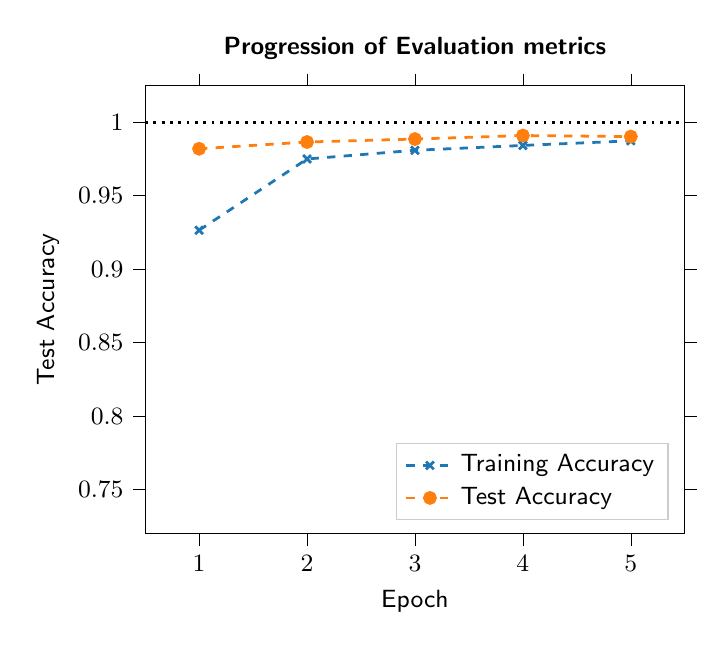
\begin{tikzpicture}

\definecolor{color0}{rgb}{0.12156862745098,0.466666666666667,0.705882352941177}
\definecolor{color1}{rgb}{1,0.498039215686275,0.0549019607843137}

\begin{axis}[
font=\small,
legend cell align={left},
legend style={at={(0.97,0.03)}, anchor=south east, draw=white!80.0!black},
minor xtick={},
minor ytick={},
tick align=outside,
tick pos=both,
title={{\bf Progression of Evaluation metrics}},
x grid style={white!69.01960784313725!black},
xlabel={Epoch},
xmin=0.5, xmax=5.5,
xtick style={color=black},
xtick={1,2,3,4,5},
y grid style={white!69.01960784313725!black},
ylabel={Test Accuracy},
ymin=0.72, ymax=1.025,
ytick style={color=black},
ytick={0.7,0.75,0.8,0.85,0.9,0.95,1,1.05}
]
\addplot [line width=1.0pt, color0, dashed, mark=x, mark size=2, mark options={solid}]
table {%
1 0.926466666666667
2 0.97495
3 0.980866666698456
4 0.984166666698456
5 0.987300000031789
};
\addlegendentry{Training Accuracy}
\addplot [line width=1.0pt, color1, dashed, mark=*, mark size=2, mark options={solid}]
table {%
1 0.9819
2 0.9865
3 0.9885
4 0.9909
5 0.9902
};
\addlegendentry{Test Accuracy}
\addplot [line width=1.0pt, black, dotted, forget plot]
table {%
0.5 1
5.5 1
};
\end{axis}

\end{tikzpicture}
            \caption{Accuracy learning process for model \protect\hyperref[training:2]
                        {2}.}
        \end{subfigure}%
        \hfill%
        \begin{subfigure}{.5\textwidth}
            % This file was created by tikzplotlib v0.8.2.
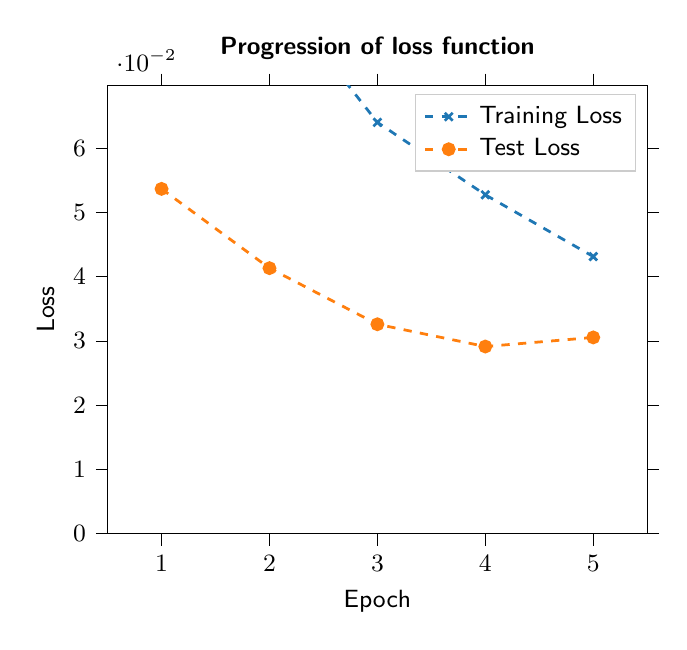
\begin{tikzpicture}

\definecolor{color0}{rgb}{0.12156862745098,0.466666666666667,0.705882352941177}
\definecolor{color1}{rgb}{1,0.498039215686275,0.0549019607843137}

\begin{axis}[
font=\small,
legend cell align={left},
legend style={draw=white!80.0!black},
minor xtick={},
minor ytick={},
tick align=outside,
tick pos=both,
title={{\bf Progression of loss function}},
x grid style={white!69.01960784313725!black},
xlabel={Epoch},
xmin=0.5, xmax=5.5,
xtick style={color=black},
xtick={1,2,3,4,5},
y grid style={white!69.01960784313725!black},
ylabel={Loss},
ymin=0, ymax=0.0697562867802568,
ytick style={color=black},
ytick={0,0.01,0.02,0.03,0.04,0.05,0.06,0.07}
]
\addplot [line width=1.0pt, color0, dashed, mark=x, mark size=2, mark options={solid}]
table {%
1 0.241077901148796
2 0.0853335331380367
3 0.0640075407187144
4 0.0527333358973265
5 0.0431256611426671
};
\addlegendentry{Training Loss}
\addplot [line width=1.0pt, color1, dashed, mark=*, mark size=2, mark options={solid}]
table {%
1 0.0536586821386591
2 0.0413232616130728
3 0.0325934046631679
4 0.02912832682851
5 0.0305453931855271
};
\addlegendentry{Test Loss}
\end{axis}

\end{tikzpicture}
            \caption{Loss learning process for model \protect\hyperref[training:2]
                        {2}.}
        \end{subfigure}
        \par\bigskip
        \begin{subfigure}{.5\textwidth}
            % This file was created by tikzplotlib v0.8.2.
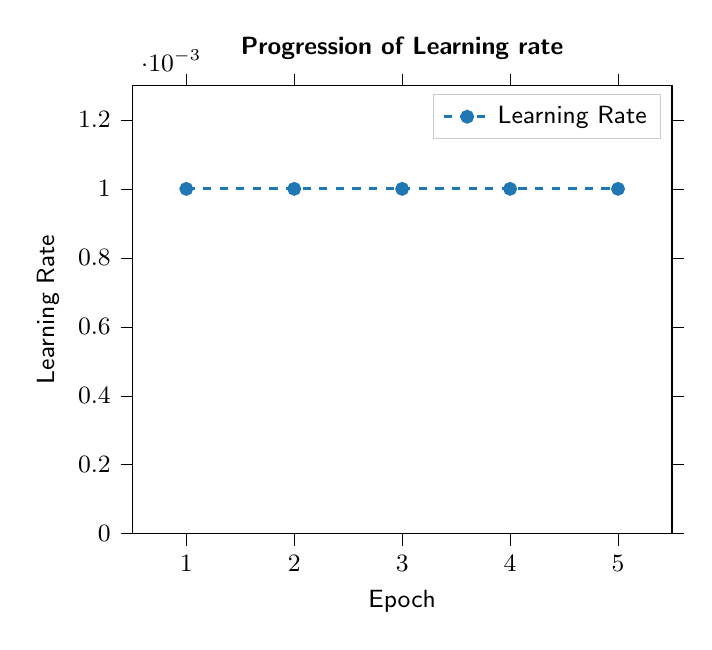
\begin{tikzpicture}

\definecolor{color0}{rgb}{0.12156862745098,0.466666666666667,0.705882352941177}

\begin{axis}[
font=\small,
legend cell align={left},
legend style={draw=white!80.0!black},
minor xtick={},
minor ytick={},
tick align=outside,
tick pos=both,
title={{\bf Progression of Learning rate}},
x grid style={white!69.01960784313725!black},
xlabel={Epoch},
xmin=0.5, xmax=5.5,
xtick style={color=black},
xtick={1,2,3,4,5},
y grid style={white!69.01960784313725!black},
ylabel={Learning Rate},
ymin=0, ymax=0.0013,
ytick style={color=black},
ytick={0,0.0002,0.0004,0.0006,0.0008,0.001,0.0012,0.0014}
]
\addplot [line width=1.0pt, color0, dashed, mark=*, mark size=2, mark options={solid}]
table {%
1 0.001
2 0.001
3 0.001
4 0.001
5 0.001
};
\addlegendentry{Learning Rate}
\end{axis}

\end{tikzpicture}
            \caption{Learning rate per epoch for model \protect\hyperref[training:2]
                        {2}.}
        \end{subfigure}%
        \caption{Training and evaluation metrics for model  \protect\hyperref[training:2]
                    {2}.
                \label{fig:results2}}
    \end{figure}

    \subsubsection*{Dataset}
    \begin{description}
        \item[Name] MNIST
        \item[Train-Test-Dev split:] {\it Training set:}
        60000,
        {\it Test set:}
        10000,
        {\it Dev set:}
        0,
        \item[Image size] [28, 28]


    \end{description}
    %
    \subsubsection*{Training}
    \begin{description}
        \item[Number of epochs] 5
        \item[Optimizer] Adam (Kingma et al., 2015)

            \begin{tabular}{rl}
                    {\bf Learning Rate} & 0.0010000000474974513 \\
                    {\bf Beta 1} & 0.8999999761581421 \\
                    {\bf Beta 2} & 0.9990000128746033 \\
                    {\bf Decay} & 0.0 \\
                    {\bf Epsilon} & 1e-07 \\
                    {\bf Amsgrad} & False \\
            \end{tabular}

        \item[Loss] Categorical crossentropy
        \item[Batch size] 128
        \item[Shuffle] Yes
        \item[Training time] 39 sec
    \end{description}
    %
    \subsubsection*{Platform}
    \begin{description}
        \item[Weights exported to path] weights\textbackslash ConvNet2layers\_5ep\_MNIST.h5
        \item[Device used] GPU (GeForce GTX 1060 6GB)
        \item[CPU] Intel(R) Xeon(R) CPU E3-1245 v5 @ 3.50GHz,
                   X86\_64
        \item[Python Version] 3.7.2.final.0 (64 bit)
        \item[Keras Version] 2.2.5 (Backend: tensorflow)
        \item[Tensorflow Version] 1.14.0
        \item[Timestamp] 25.09.2019 at 16:04
    \end{description}
    \subsection{Model 3:
                        ConvNet2layers
                \label{training:3}
                }
    %
    \paragraph*{Training history} See Figure \ref{fig:results3}.
    \begin{figure}[H]
        \centering
        \begin{subfigure}{.5\textwidth}
            % This file was created by tikzplotlib v0.8.2.
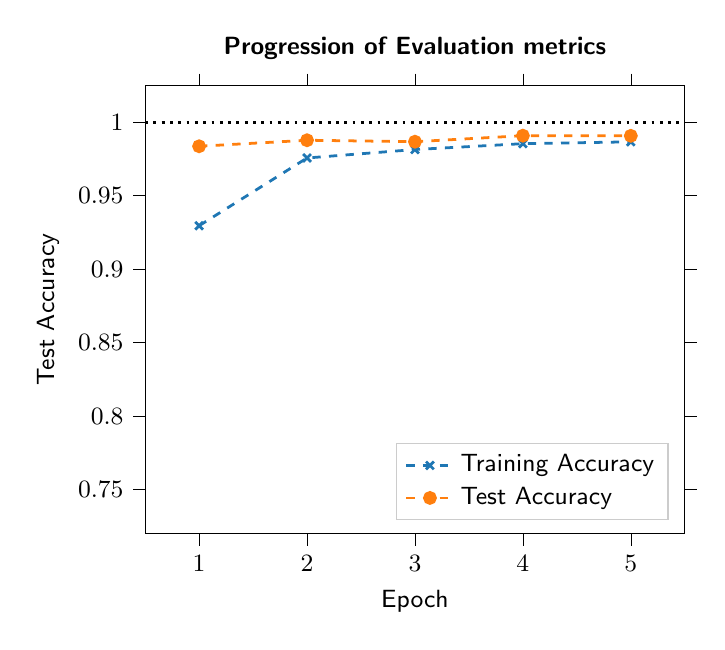
\begin{tikzpicture}

\definecolor{color0}{rgb}{0.12156862745098,0.466666666666667,0.705882352941177}
\definecolor{color1}{rgb}{1,0.498039215686275,0.0549019607843137}

\begin{axis}[
font=\small,
legend cell align={left},
legend style={at={(0.97,0.03)}, anchor=south east, draw=white!80.0!black},
minor xtick={},
minor ytick={},
tick align=outside,
tick pos=both,
title={{\bf Progression of Evaluation metrics}},
x grid style={white!69.01960784313725!black},
xlabel={Epoch},
xmin=0.5, xmax=5.5,
xtick style={color=black},
xtick={1,2,3,4,5},
y grid style={white!69.01960784313725!black},
ylabel={Test Accuracy},
ymin=0.72, ymax=1.025,
ytick style={color=black},
ytick={0.7,0.75,0.8,0.85,0.9,0.95,1,1.05}
]
\addplot [line width=1.0pt, color0, dashed, mark=x, mark size=2, mark options={solid}]
table {%
1 0.929533333333333
2 0.975633333365122
3 0.981383333301544
4 0.985366666698456
5 0.986616666666667
};
\addlegendentry{Training Accuracy}
\addplot [line width=1.0pt, color1, dashed, mark=*, mark size=2, mark options={solid}]
table {%
1 0.9836
2 0.9877
3 0.9867
4 0.9908
5 0.9907
};
\addlegendentry{Test Accuracy}
\addplot [line width=1.0pt, black, dotted, forget plot]
table {%
0.5 1
5.5 1
};
\end{axis}

\end{tikzpicture}
            \caption{Accuracy learning process for model \protect\hyperref[training:3]
                        {3}.}
        \end{subfigure}%
        \hfill%
        \begin{subfigure}{.5\textwidth}
            % This file was created by tikzplotlib v0.8.2.
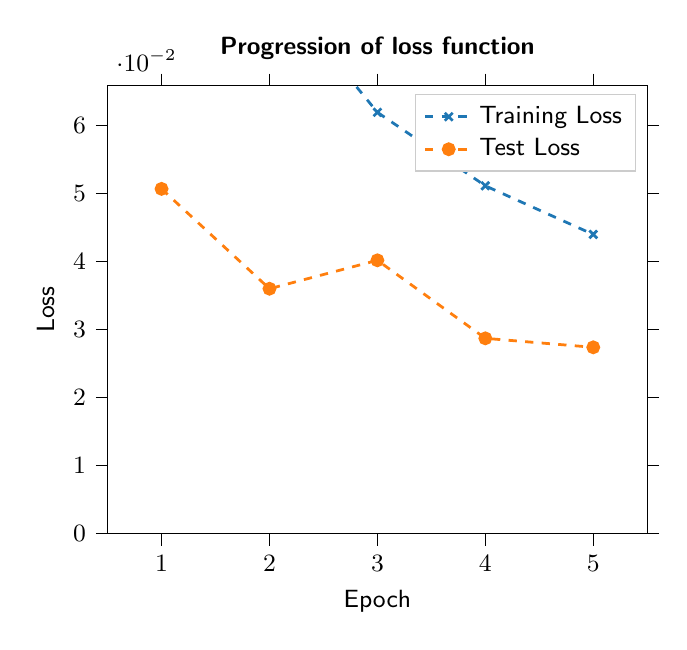
\begin{tikzpicture}

\definecolor{color0}{rgb}{0.12156862745098,0.466666666666667,0.705882352941177}
\definecolor{color1}{rgb}{1,0.498039215686275,0.0549019607843137}

\begin{axis}[
font=\small,
legend cell align={left},
legend style={draw=white!80.0!black},
minor xtick={},
minor ytick={},
tick align=outside,
tick pos=both,
title={{\bf Progression of loss function}},
x grid style={white!69.01960784313725!black},
xlabel={Epoch},
xmin=0.5, xmax=5.5,
xtick style={color=black},
xtick={1,2,3,4,5},
y grid style={white!69.01960784313725!black},
ylabel={Loss},
ymin=0, ymax=0.0659350888817757,
ytick style={color=black},
ytick={0,0.01,0.02,0.03,0.04,0.05,0.06,0.07}
]
\addplot [line width=1.0pt, color0, dashed, mark=x, mark size=2, mark options={solid}]
table {%
1 0.231233902275562
2 0.0813334892590841
3 0.0619803109814723
4 0.0511684121588866
5 0.0440221101800601
};
\addlegendentry{Training Loss}
\addplot [line width=1.0pt, color1, dashed, mark=*, mark size=2, mark options={solid}]
table {%
1 0.0507192991398275
2 0.0360333215791732
3 0.0402135029521305
4 0.0287386026042048
5 0.0274173404738773
};
\addlegendentry{Test Loss}
\end{axis}

\end{tikzpicture}
            \caption{Loss learning process for model \protect\hyperref[training:3]
                        {3}.}
        \end{subfigure}
        \par\bigskip
        \begin{subfigure}{.5\textwidth}
            % This file was created by tikzplotlib v0.8.2.
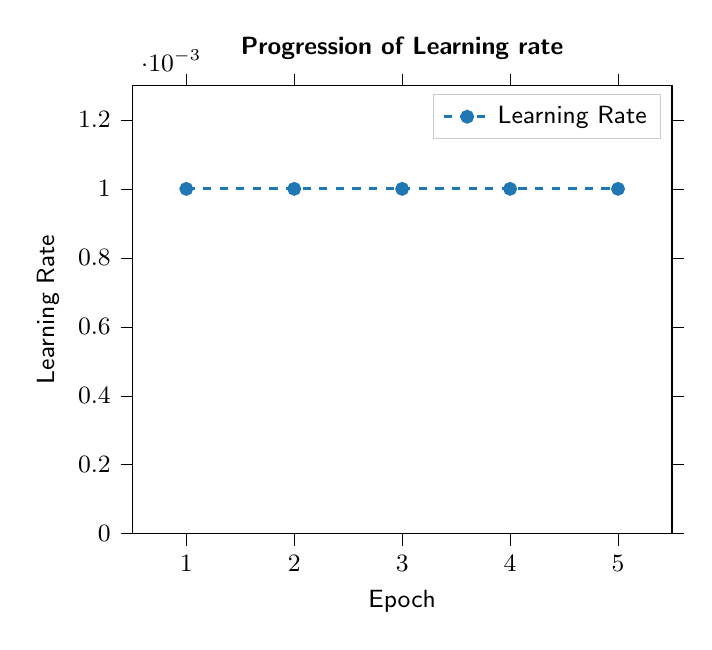
\begin{tikzpicture}

\definecolor{color0}{rgb}{0.12156862745098,0.466666666666667,0.705882352941177}

\begin{axis}[
font=\small,
legend cell align={left},
legend style={draw=white!80.0!black},
minor xtick={},
minor ytick={},
tick align=outside,
tick pos=both,
title={{\bf Progression of Learning rate}},
x grid style={white!69.01960784313725!black},
xlabel={Epoch},
xmin=0.5, xmax=5.5,
xtick style={color=black},
xtick={1,2,3,4,5},
y grid style={white!69.01960784313725!black},
ylabel={Learning Rate},
ymin=0, ymax=0.0013,
ytick style={color=black},
ytick={0,0.0002,0.0004,0.0006,0.0008,0.001,0.0012,0.0014}
]
\addplot [line width=1.0pt, color0, dashed, mark=*, mark size=2, mark options={solid}]
table {%
1 0.001
2 0.001
3 0.001
4 0.001
5 0.001
};
\addlegendentry{Learning Rate}
\end{axis}

\end{tikzpicture}
            \caption{Learning rate per epoch for model \protect\hyperref[training:3]
                        {3}.}
        \end{subfigure}%
        \caption{Training and evaluation metrics for model  \protect\hyperref[training:3]
                    {3}.
                \label{fig:results3}}
    \end{figure}

    \subsubsection*{Dataset}
    \begin{description}
        \item[Name] MNIST
        \item[Train-Test-Dev split:] {\it Training set:}
        60000,
        {\it Test set:}
        10000,
        {\it Dev set:}
        0,
        \item[Image size] [28, 28]


    \end{description}
    %
    \subsubsection*{Training}
    \begin{description}
        \item[Number of epochs] 5
        \item[Optimizer] Adam (Kingma et al., 2015)

            \begin{tabular}{rl}
                    {\bf Learning Rate} & 0.0010000000474974513 \\
                    {\bf Beta 1} & 0.8999999761581421 \\
                    {\bf Beta 2} & 0.9990000128746033 \\
                    {\bf Decay} & 0.0 \\
                    {\bf Epsilon} & 1e-07 \\
                    {\bf Amsgrad} & False \\
            \end{tabular}

        \item[Loss] Categorical crossentropy
        \item[Batch size] 128
        \item[Shuffle] Yes
        \item[Training time] 36 sec
    \end{description}
    %
    \subsubsection*{Platform}
    \begin{description}
        \item[Weights exported to path] weights\textbackslash ConvNet2layers\_5ep\_MNIST.h5
        \item[Device used] GPU (GeForce GTX 1060 6GB)
        \item[CPU] Intel(R) Xeon(R) CPU E3-1245 v5 @ 3.50GHz,
                   X86\_64
        \item[Python Version] 3.7.2.final.0 (64 bit)
        \item[Keras Version] 2.2.5 (Backend: tensorflow)
        \item[Tensorflow Version] 1.14.0
        \item[Timestamp] 25.09.2019 at 16:07
    \end{description}
    \subsection{Model 4:
                        ConvNet2layers
                \label{training:4}
                }
    %
    \paragraph*{Training history} See Figure \ref{fig:results4}.
    \begin{figure}[H]
        \centering
        \begin{subfigure}{.5\textwidth}
            % This file was created by tikzplotlib v0.8.2.
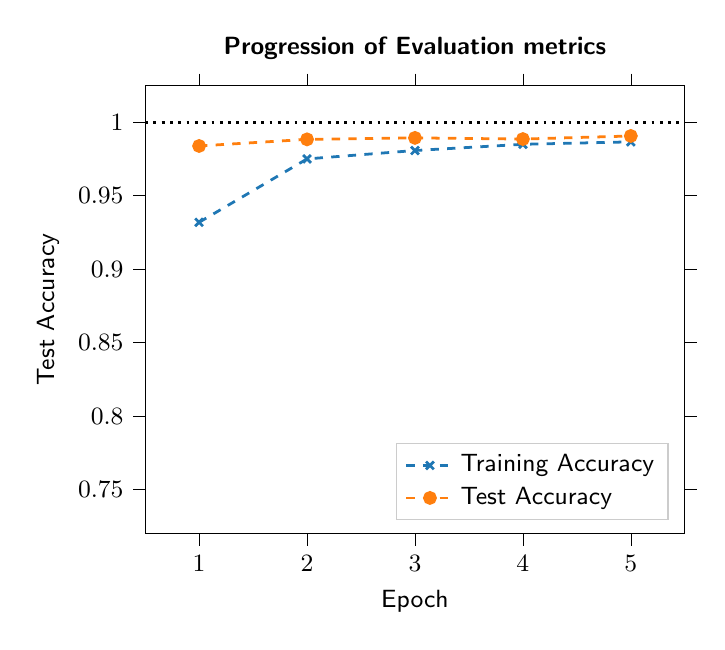
\begin{tikzpicture}

\definecolor{color0}{rgb}{0.12156862745098,0.466666666666667,0.705882352941177}
\definecolor{color1}{rgb}{1,0.498039215686275,0.0549019607843137}

\begin{axis}[
font=\small,
legend cell align={left},
legend style={at={(0.97,0.03)}, anchor=south east, draw=white!80.0!black},
minor xtick={},
minor ytick={},
tick align=outside,
tick pos=both,
title={{\bf Progression of Evaluation metrics}},
x grid style={white!69.01960784313725!black},
xlabel={Epoch},
xmin=0.5, xmax=5.5,
xtick style={color=black},
xtick={1,2,3,4,5},
y grid style={white!69.01960784313725!black},
ylabel={Test Accuracy},
ymin=0.72, ymax=1.025,
ytick style={color=black},
ytick={0.7,0.75,0.8,0.85,0.9,0.95,1,1.05}
]
\addplot [line width=1.0pt, color0, dashed, mark=x, mark size=2, mark options={solid}]
table {%
1 0.931866666698456
2 0.975
3 0.980716666666667
4 0.984933333301544
5 0.986599999968211
};
\addlegendentry{Training Accuracy}
\addplot [line width=1.0pt, color1, dashed, mark=*, mark size=2, mark options={solid}]
table {%
1 0.9838
2 0.9883
3 0.9893
4 0.9885
5 0.9906
};
\addlegendentry{Test Accuracy}
\addplot [line width=1.0pt, black, dotted, forget plot]
table {%
0.5 1
5.5 1
};
\end{axis}

\end{tikzpicture}
            \caption{Accuracy learning process for model \protect\hyperref[training:4]
                        {4}.}
        \end{subfigure}%
        \hfill%
        \begin{subfigure}{.5\textwidth}
            % This file was created by tikzplotlib v0.8.2.
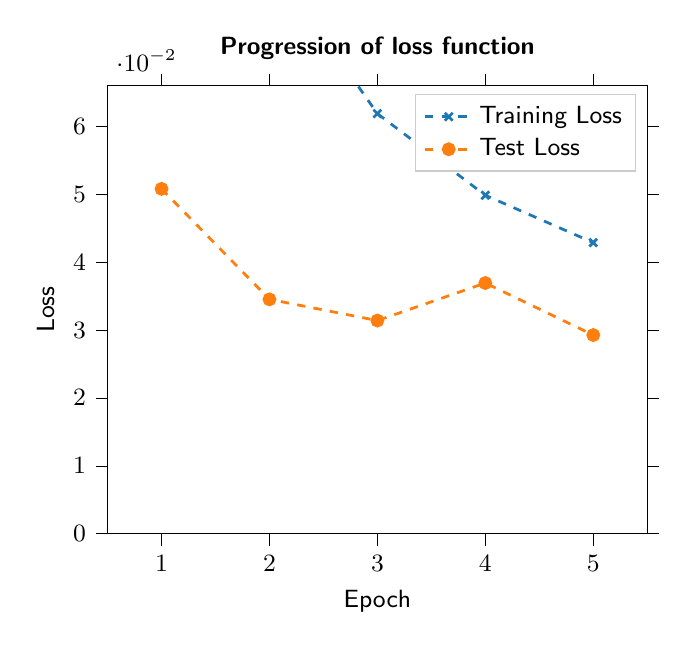
\begin{tikzpicture}

\definecolor{color0}{rgb}{0.12156862745098,0.466666666666667,0.705882352941177}
\definecolor{color1}{rgb}{1,0.498039215686275,0.0549019607843137}

\begin{axis}[
font=\small,
legend cell align={left},
legend style={draw=white!80.0!black},
minor xtick={},
minor ytick={},
tick align=outside,
tick pos=both,
title={{\bf Progression of loss function}},
x grid style={white!69.01960784313725!black},
xlabel={Epoch},
xmin=0.5, xmax=5.5,
xtick style={color=black},
xtick={1,2,3,4,5},
y grid style={white!69.01960784313725!black},
ylabel={Loss},
ymin=0, ymax=0.0660322530353721,
ytick style={color=black},
ytick={0,0.01,0.02,0.03,0.04,0.05,0.06,0.07}
]
\addplot [line width=1.0pt, color0, dashed, mark=x, mark size=2, mark options={solid}]
table {%
1 0.224691664151351
2 0.0845302988529205
3 0.0618758745615681
4 0.0498506396760543
5 0.0428804140528043
};
\addlegendentry{Training Loss}
\addplot [line width=1.0pt, color1, dashed, mark=*, mark size=2, mark options={solid}]
table {%
1 0.0507940407964401
2 0.0345216840307228
3 0.0313966272048187
4 0.0369274285364314
5 0.029261906390707
};
\addlegendentry{Test Loss}
\end{axis}

\end{tikzpicture}
            \caption{Loss learning process for model \protect\hyperref[training:4]
                        {4}.}
        \end{subfigure}
        \par\bigskip
        \begin{subfigure}{.5\textwidth}
            % This file was created by tikzplotlib v0.8.2.
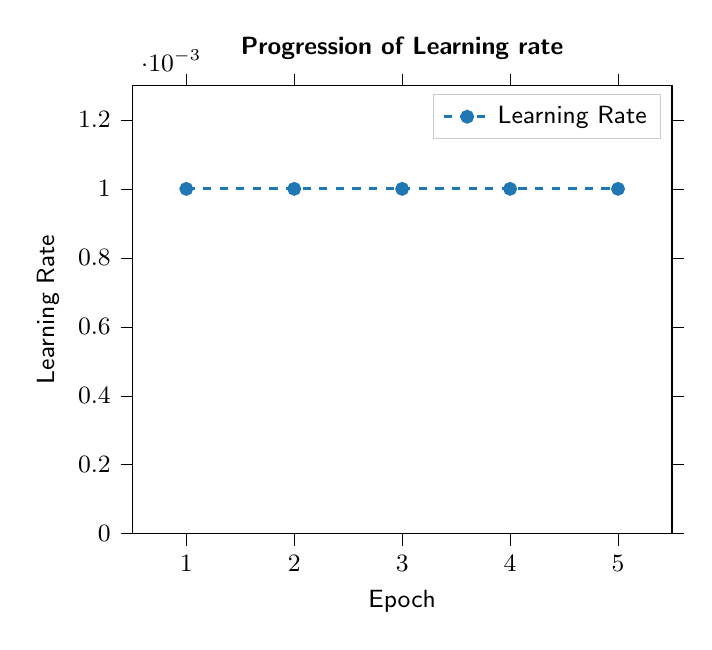
\begin{tikzpicture}

\definecolor{color0}{rgb}{0.12156862745098,0.466666666666667,0.705882352941177}

\begin{axis}[
font=\small,
legend cell align={left},
legend style={draw=white!80.0!black},
minor xtick={},
minor ytick={},
tick align=outside,
tick pos=both,
title={{\bf Progression of Learning rate}},
x grid style={white!69.01960784313725!black},
xlabel={Epoch},
xmin=0.5, xmax=5.5,
xtick style={color=black},
xtick={1,2,3,4,5},
y grid style={white!69.01960784313725!black},
ylabel={Learning Rate},
ymin=0, ymax=0.0013,
ytick style={color=black},
ytick={0,0.0002,0.0004,0.0006,0.0008,0.001,0.0012,0.0014}
]
\addplot [line width=1.0pt, color0, dashed, mark=*, mark size=2, mark options={solid}]
table {%
1 0.001
2 0.001
3 0.001
4 0.001
5 0.001
};
\addlegendentry{Learning Rate}
\end{axis}

\end{tikzpicture}
            \caption{Learning rate per epoch for model \protect\hyperref[training:4]
                        {4}.}
        \end{subfigure}%
        \caption{Training and evaluation metrics for model  \protect\hyperref[training:4]
                    {4}.
                \label{fig:results4}}
    \end{figure}

    \subsubsection*{Dataset}
    \begin{description}
        \item[Name] MNIST
        \item[Train-Test-Dev split:] {\it Training set:}
        60000,
        {\it Test set:}
        10000,
        {\it Dev set:}
        0,
        \item[Image size] [28, 28]


    \end{description}
    %
    \subsubsection*{Training}
    \begin{description}
        \item[Number of epochs] 5
        \item[Optimizer] Adam (Kingma et al., 2015)

            \begin{tabular}{rl}
                    {\bf Learning Rate} & 0.0010000000474974513 \\
                    {\bf Beta 1} & 0.8999999761581421 \\
                    {\bf Beta 2} & 0.9990000128746033 \\
                    {\bf Decay} & 0.0 \\
                    {\bf Epsilon} & 1e-07 \\
                    {\bf Amsgrad} & False \\
            \end{tabular}

        \item[Loss] Categorical crossentropy
        \item[Batch size] 128
        \item[Shuffle] Yes
        \item[Training time] 39 sec
    \end{description}
    %
    \subsubsection*{Platform}
    \begin{description}
        \item[Weights exported to path] weights\textbackslash ConvNet2layers\_5ep\_MNIST.h5
        \item[Device used] GPU (GeForce GTX 1060 6GB)
        \item[CPU] Intel(R) Xeon(R) CPU E3-1245 v5 @ 3.50GHz,
                   X86\_64
        \item[Python Version] 3.7.2.final.0 (64 bit)
        \item[Keras Version] 2.2.5 (Backend: tensorflow)
        \item[Tensorflow Version] 1.14.0
        \item[Timestamp] 25.09.2019 at 16:10
    \end{description}
    \subsection{Model 5:
                        MLP2layers
                \label{training:5}
                }
    %
    \paragraph*{Training history} See Figure \ref{fig:results5}.
    \begin{figure}[H]
        \centering
        \begin{subfigure}{.5\textwidth}
            % This file was created by tikzplotlib v0.8.2.
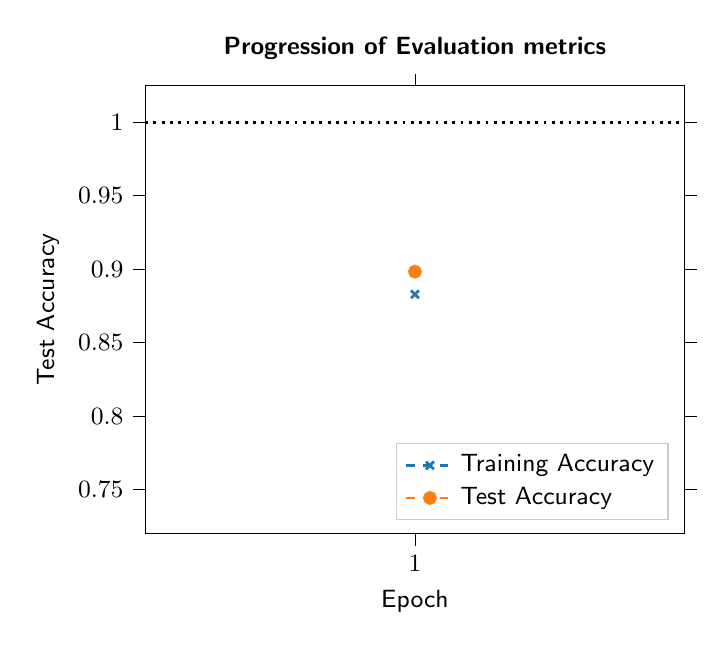
\begin{tikzpicture}

\definecolor{color0}{rgb}{0.12156862745098,0.466666666666667,0.705882352941177}
\definecolor{color1}{rgb}{1,0.498039215686275,0.0549019607843137}

\begin{axis}[
font=\small,
legend cell align={left},
legend style={at={(0.97,0.03)}, anchor=south east, draw=white!80.0!black},
minor xtick={},
minor ytick={},
tick align=outside,
tick pos=both,
title={{\bf Progression of Evaluation metrics}},
x grid style={white!69.01960784313725!black},
xlabel={Epoch},
xmin=0.5, xmax=1.5,
xtick style={color=black},
xtick={1},
y grid style={white!69.01960784313725!black},
ylabel={Test Accuracy},
ymin=0.72, ymax=1.025,
ytick style={color=black},
ytick={0.7,0.75,0.8,0.85,0.9,0.95,1,1.05}
]
\addplot [line width=1.0pt, color0, dashed, mark=x, mark size=2, mark options={solid}]
table {%
1 0.882916666634878
};
\addlegendentry{Training Accuracy}
\addplot [line width=1.0pt, color1, dashed, mark=*, mark size=2, mark options={solid}]
table {%
1 0.8983
};
\addlegendentry{Test Accuracy}
\addplot [line width=1.0pt, black, dotted, forget plot]
table {%
0.5 1
1.5 1
};
\end{axis}

\end{tikzpicture}
            \caption{Accuracy learning process for model \protect\hyperref[training:5]
                        {5}.}
        \end{subfigure}%
        \hfill%
        \begin{subfigure}{.5\textwidth}
            % This file was created by tikzplotlib v0.8.2.
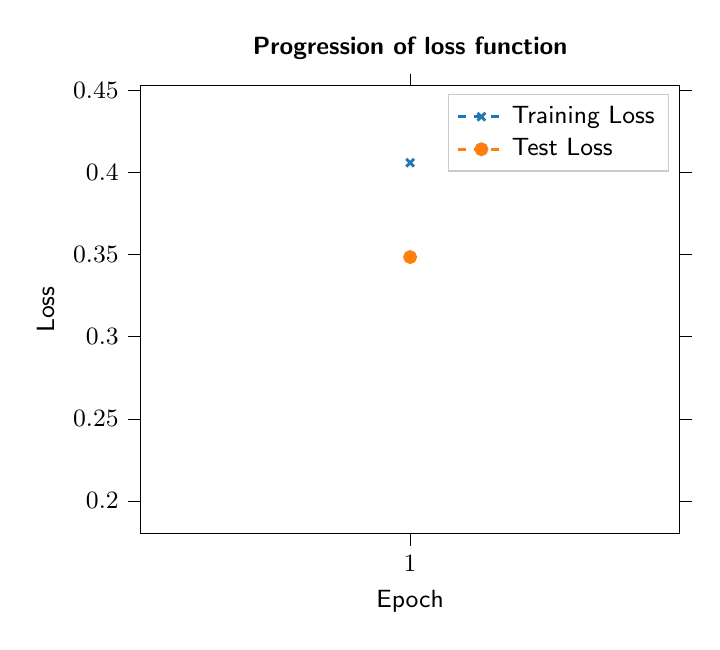
\begin{tikzpicture}

\definecolor{color0}{rgb}{0.12156862745098,0.466666666666667,0.705882352941177}
\definecolor{color1}{rgb}{1,0.498039215686275,0.0549019607843137}

\begin{axis}[
font=\small,
legend cell align={left},
legend style={draw=white!80.0!black},
minor xtick={},
minor ytick={},
tick align=outside,
tick pos=both,
title={{\bf Progression of loss function}},
x grid style={white!69.01960784313725!black},
xlabel={Epoch},
xmin=0.5, xmax=1.5,
xtick style={color=black},
xtick={1},
y grid style={white!69.01960784313725!black},
ylabel={Loss},
ymin=0.18, ymax=0.453106989803314,
ytick style={color=black},
ytick={0.15,0.2,0.25,0.3,0.35,0.4,0.45,0.5}
]
\addplot [line width=1.0pt, color0, dashed, mark=x, mark size=2, mark options={solid}]
table {%
1 0.405979485925039
};
\addlegendentry{Training Loss}
\addplot [line width=1.0pt, color1, dashed, mark=*, mark size=2, mark options={solid}]
table {%
1 0.348543838310242
};
\addlegendentry{Test Loss}
\end{axis}

\end{tikzpicture}
            \caption{Loss learning process for model \protect\hyperref[training:5]
                        {5}.}
        \end{subfigure}
        \par\bigskip
        \begin{subfigure}{.5\textwidth}
            % This file was created by tikzplotlib v0.8.2.
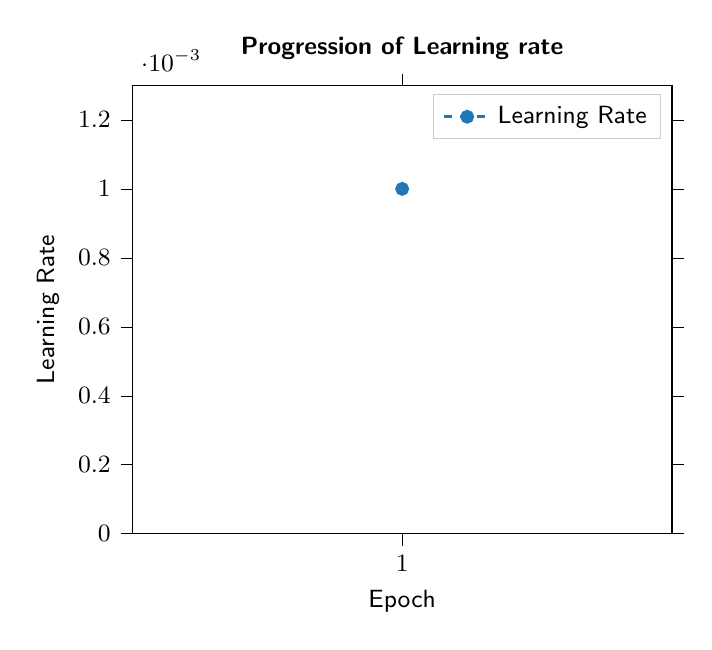
\begin{tikzpicture}

\definecolor{color0}{rgb}{0.12156862745098,0.466666666666667,0.705882352941177}

\begin{axis}[
font=\small,
legend cell align={left},
legend style={draw=white!80.0!black},
minor xtick={},
minor ytick={},
tick align=outside,
tick pos=both,
title={{\bf Progression of Learning rate}},
x grid style={white!69.01960784313725!black},
xlabel={Epoch},
xmin=0.5, xmax=1.5,
xtick style={color=black},
xtick={1},
y grid style={white!69.01960784313725!black},
ylabel={Learning Rate},
ymin=0, ymax=0.0013,
ytick style={color=black},
ytick={0,0.0002,0.0004,0.0006,0.0008,0.001,0.0012,0.0014}
]
\addplot [line width=1.0pt, color0, dashed, mark=*, mark size=2, mark options={solid}]
table {%
1 0.001
};
\addlegendentry{Learning Rate}
\end{axis}

\end{tikzpicture}
            \caption{Learning rate per epoch for model \protect\hyperref[training:5]
                        {5}.}
        \end{subfigure}%
        \caption{Training and evaluation metrics for model  \protect\hyperref[training:5]
                    {5}.
                \label{fig:results5}}
    \end{figure}

    \subsubsection*{Dataset}
    \begin{description}
        \item[Name] MNIST
        \item[Train-Test-Dev split:] {\it Training set:}
        60000,
        {\it Test set:}
        10000,
        {\it Dev set:}
        0,
        \item[Image size] [28, 28]


    \end{description}
    %
    \subsubsection*{Training}
    \begin{description}
        \item[Number of epochs] 1
        \item[Optimizer] Adam (Kingma et al., 2015)

            \begin{tabular}{rl}
                    {\bf Learning Rate} & 0.0010000000474974513 \\
                    {\bf Beta 1} & 0.8999999761581421 \\
                    {\bf Beta 2} & 0.9990000128746033 \\
                    {\bf Decay} & 0.0 \\
                    {\bf Epsilon} & 1e-07 \\
                    {\bf Amsgrad} & False \\
            \end{tabular}

        \item[Loss] Categorical crossentropy
        \item[Batch size] 128
        \item[Shuffle] Yes
        \item[Training time] 5 sec
    \end{description}
    %
    \subsubsection*{Platform}
    \begin{description}
        \item[Weights exported to path] weights\textbackslash MLP2layers\_1ep\_MNIST.h5
        \item[Device used] GPU (GeForce GTX 1060 6GB)
        \item[CPU] Intel(R) Xeon(R) CPU E3-1245 v5 @ 3.50GHz,
                   X86\_64
        \item[Python Version] 3.7.2.final.0 (64 bit)
        \item[Keras Version] 2.2.5 (Backend: tensorflow)
        \item[Tensorflow Version] 1.14.0
        \item[Timestamp] 25.09.2019 at 15:16
    \end{description}
    \subsection{Model 6:
                        MLP2layers
                \label{training:6}
                }
    %
    \paragraph*{Training history} See Figure \ref{fig:results6}.
    \begin{figure}[H]
        \centering
        \begin{subfigure}{.5\textwidth}
            % This file was created by tikzplotlib v0.8.2.
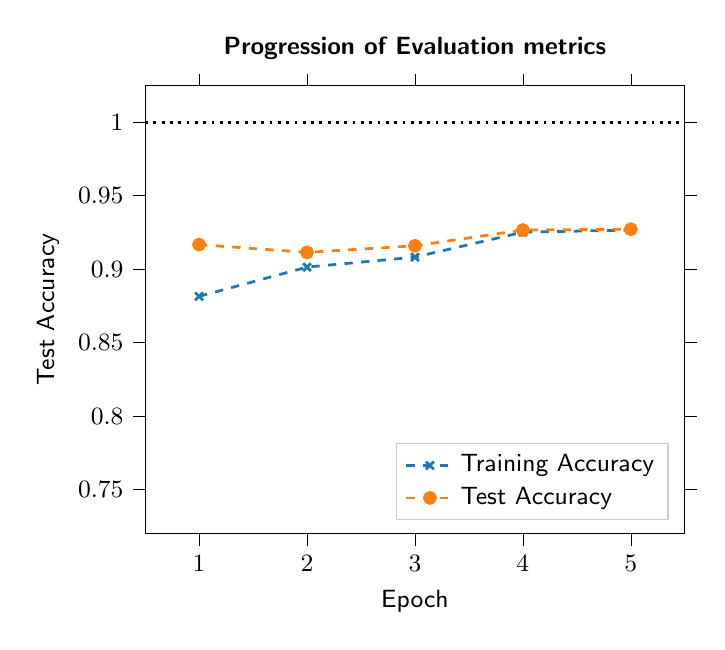
\begin{tikzpicture}

\definecolor{color0}{rgb}{0.12156862745098,0.466666666666667,0.705882352941177}
\definecolor{color1}{rgb}{1,0.498039215686275,0.0549019607843137}

\begin{axis}[
font=\small,
legend cell align={left},
legend style={at={(0.97,0.03)}, anchor=south east, draw=white!80.0!black},
minor xtick={},
minor ytick={},
tick align=outside,
tick pos=both,
title={{\bf Progression of Evaluation metrics}},
x grid style={white!69.01960784313725!black},
xlabel={Epoch},
xmin=0.5, xmax=5.5,
xtick style={color=black},
xtick={1,2,3,4,5},
y grid style={white!69.01960784313725!black},
ylabel={Test Accuracy},
ymin=0.72, ymax=1.025,
ytick style={color=black},
ytick={0.7,0.75,0.8,0.85,0.9,0.95,1,1.05}
]
\addplot [line width=1.0pt, color0, dashed, mark=x, mark size=2, mark options={solid}]
table {%
1 0.881499999968211
2 0.901383333365122
3 0.908183333333333
4 0.925150000031789
5 0.926600000031789
};
\addlegendentry{Training Accuracy}
\addplot [line width=1.0pt, color1, dashed, mark=*, mark size=2, mark options={solid}]
table {%
1 0.9167
2 0.9114
3 0.9159
4 0.9266
5 0.9272
};
\addlegendentry{Test Accuracy}
\addplot [line width=1.0pt, black, dotted, forget plot]
table {%
0.5 1
5.5 1
};
\end{axis}

\end{tikzpicture}
            \caption{Accuracy learning process for model \protect\hyperref[training:6]
                        {6}.}
        \end{subfigure}%
        \hfill%
        \begin{subfigure}{.5\textwidth}
            % This file was created by tikzplotlib v0.8.2.
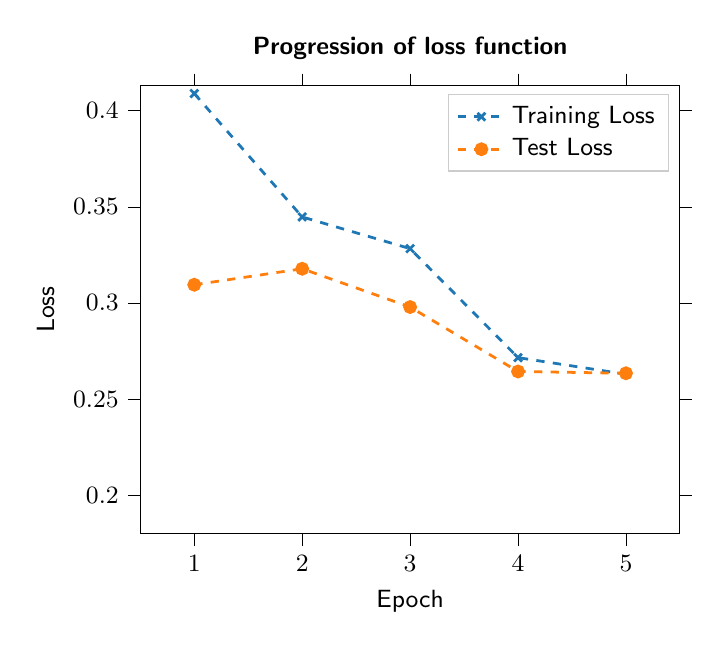
\begin{tikzpicture}

\definecolor{color0}{rgb}{0.12156862745098,0.466666666666667,0.705882352941177}
\definecolor{color1}{rgb}{1,0.498039215686275,0.0549019607843137}

\begin{axis}[
font=\small,
legend cell align={left},
legend style={draw=white!80.0!black},
minor xtick={},
minor ytick={},
tick align=outside,
tick pos=both,
title={{\bf Progression of loss function}},
x grid style={white!69.01960784313725!black},
xlabel={Epoch},
xmin=0.5, xmax=5.5,
xtick style={color=black},
xtick={1,2,3,4,5},
y grid style={white!69.01960784313725!black},
ylabel={Loss},
ymin=0.18, ymax=0.413102377243042,
ytick style={color=black},
ytick={0.15,0.2,0.25,0.3,0.35,0.4,0.45}
]
\addplot [line width=1.0pt, color0, dashed, mark=x, mark size=2, mark options={solid}]
table {%
1 0.408876964362462
2 0.344722838640213
3 0.328236488644282
4 0.271567789745331
5 0.262939639091492
};
\addlegendentry{Training Loss}
\addplot [line width=1.0pt, color1, dashed, mark=*, mark size=2, mark options={solid}]
table {%
1 0.309456143224239
2 0.317771059417725
3 0.297867096781731
4 0.264359930229187
5 0.263443100523949
};
\addlegendentry{Test Loss}
\end{axis}

\end{tikzpicture}
            \caption{Loss learning process for model \protect\hyperref[training:6]
                        {6}.}
        \end{subfigure}
        \par\bigskip
        \begin{subfigure}{.5\textwidth}
            % This file was created by tikzplotlib v0.8.2.
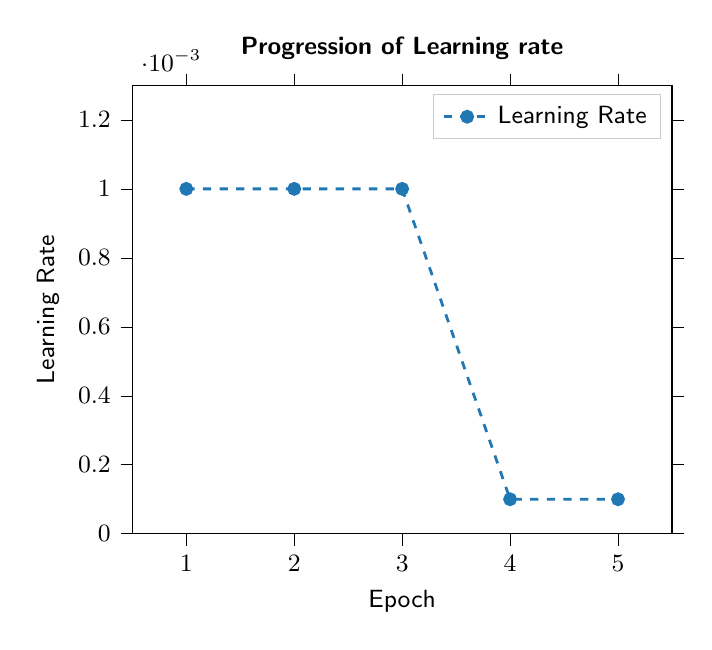
\begin{tikzpicture}

\definecolor{color0}{rgb}{0.12156862745098,0.466666666666667,0.705882352941177}

\begin{axis}[
font=\small,
legend cell align={left},
legend style={draw=white!80.0!black},
minor xtick={},
minor ytick={},
tick align=outside,
tick pos=both,
title={{\bf Progression of Learning rate}},
x grid style={white!69.01960784313725!black},
xlabel={Epoch},
xmin=0.5, xmax=5.5,
xtick style={color=black},
xtick={1,2,3,4,5},
y grid style={white!69.01960784313725!black},
ylabel={Learning Rate},
ymin=0, ymax=0.0013,
ytick style={color=black},
ytick={0,0.0002,0.0004,0.0006,0.0008,0.001,0.0012,0.0014}
]
\addplot [line width=1.0pt, color0, dashed, mark=*, mark size=2, mark options={solid}]
table {%
1 0.001
2 0.001
3 0.001
4 0.000100000005
5 0.000100000005
};
\addlegendentry{Learning Rate}
\end{axis}

\end{tikzpicture}
            \caption{Learning rate per epoch for model \protect\hyperref[training:6]
                        {6}.}
        \end{subfigure}%
        \caption{Training and evaluation metrics for model  \protect\hyperref[training:6]
                    {6}.
                \label{fig:results6}}
    \end{figure}

    \subsubsection*{Dataset}
    \begin{description}
        \item[Name] MNIST
        \item[Train-Test-Dev split:] {\it Training set:}
        60000,
        {\it Test set:}
        10000,
        {\it Dev set:}
        0,
        \item[Image size] [28, 28]


    \end{description}
    %
    \subsubsection*{Training}
    \begin{description}
        \item[Number of epochs] 5
        \item[Optimizer] Adam (Kingma et al., 2015)

            \begin{tabular}{rl}
                    {\bf Learning Rate} & 0.00010000000474974513 \\
                    {\bf Beta 1} & 0.8999999761581421 \\
                    {\bf Beta 2} & 0.9990000128746033 \\
                    {\bf Decay} & 0.0 \\
                    {\bf Epsilon} & 1e-07 \\
                    {\bf Amsgrad} & False \\
            \end{tabular}

        \item[Loss] Categorical crossentropy
        \item[Batch size] 128
        \item[Shuffle] Yes
        \item[Training time] 18 sec
    \end{description}
    %
    \subsubsection*{Platform}
    \begin{description}
        \item[Weights exported to path] weights\textbackslash MLP2layers\_5ep\_MNIST.h5
        \item[Device used] GPU (GeForce GTX 1060 6GB)
        \item[CPU] Intel(R) Xeon(R) CPU E3-1245 v5 @ 3.50GHz,
                   X86\_64
        \item[Python Version] 3.7.2.final.0 (64 bit)
        \item[Keras Version] 2.2.5 (Backend: tensorflow)
        \item[Tensorflow Version] 1.14.0
        \item[Timestamp] 25.09.2019 at 16:02
    \end{description}
    \subsection{Model 7:
                        MLP2layers
                \label{training:7}
                }
    %
    \paragraph*{Training history} See Figure \ref{fig:results7}.
    \begin{figure}[H]
        \centering
        \begin{subfigure}{.5\textwidth}
            % This file was created by tikzplotlib v0.8.2.
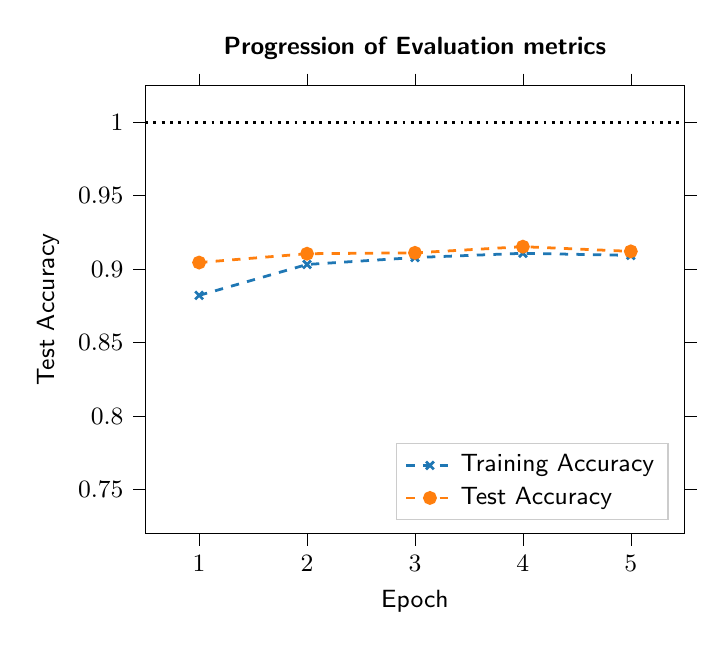
\begin{tikzpicture}

\definecolor{color0}{rgb}{0.12156862745098,0.466666666666667,0.705882352941177}
\definecolor{color1}{rgb}{1,0.498039215686275,0.0549019607843137}

\begin{axis}[
font=\small,
legend cell align={left},
legend style={at={(0.97,0.03)}, anchor=south east, draw=white!80.0!black},
minor xtick={},
minor ytick={},
tick align=outside,
tick pos=both,
title={{\bf Progression of Evaluation metrics}},
x grid style={white!69.01960784313725!black},
xlabel={Epoch},
xmin=0.5, xmax=5.5,
xtick style={color=black},
xtick={1,2,3,4,5},
y grid style={white!69.01960784313725!black},
ylabel={Test Accuracy},
ymin=0.72, ymax=1.025,
ytick style={color=black},
ytick={0.7,0.75,0.8,0.85,0.9,0.95,1,1.05}
]
\addplot [line width=1.0pt, color0, dashed, mark=x, mark size=2, mark options={solid}]
table {%
1 0.882150000031789
2 0.903183333333333
3 0.907883333301544
4 0.910783333333333
5 0.909366666698456
};
\addlegendentry{Training Accuracy}
\addplot [line width=1.0pt, color1, dashed, mark=*, mark size=2, mark options={solid}]
table {%
1 0.9045
2 0.9105
3 0.9111
4 0.9153
5 0.9121
};
\addlegendentry{Test Accuracy}
\addplot [line width=1.0pt, black, dotted, forget plot]
table {%
0.5 1
5.5 1
};
\end{axis}

\end{tikzpicture}
            \caption{Accuracy learning process for model \protect\hyperref[training:7]
                        {7}.}
        \end{subfigure}%
        \hfill%
        \begin{subfigure}{.5\textwidth}
            % This file was created by tikzplotlib v0.8.2.
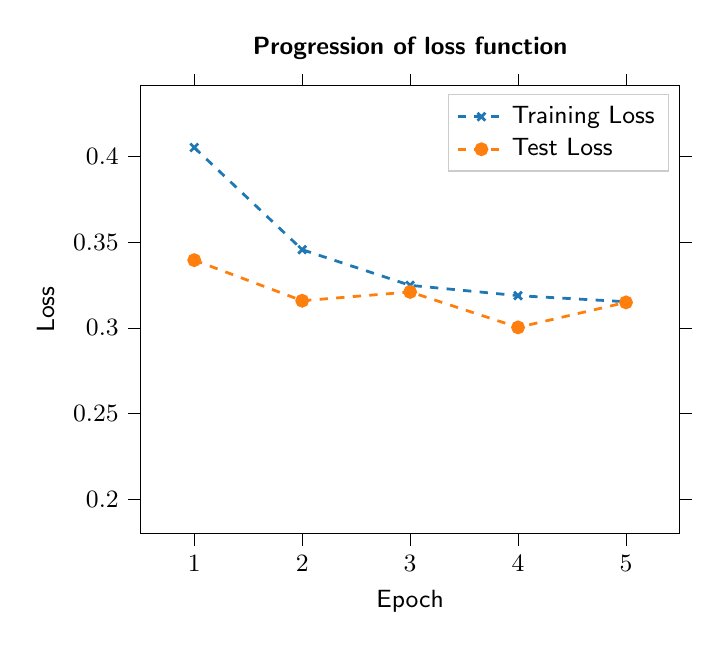
\begin{tikzpicture}

\definecolor{color0}{rgb}{0.12156862745098,0.466666666666667,0.705882352941177}
\definecolor{color1}{rgb}{1,0.498039215686275,0.0549019607843137}

\begin{axis}[
font=\small,
legend cell align={left},
legend style={draw=white!80.0!black},
minor xtick={},
minor ytick={},
tick align=outside,
tick pos=both,
title={{\bf Progression of loss function}},
x grid style={white!69.01960784313725!black},
xlabel={Epoch},
xmin=0.5, xmax=5.5,
xtick style={color=black},
xtick={1,2,3,4,5},
y grid style={white!69.01960784313725!black},
ylabel={Loss},
ymin=0.18, ymax=0.441318451590538,
ytick style={color=black},
ytick={0.15,0.2,0.25,0.3,0.35,0.4,0.45}
]
\addplot [line width=1.0pt, color0, dashed, mark=x, mark size=2, mark options={solid}]
table {%
1 0.405113116375605
2 0.345577552906672
3 0.324792588265737
4 0.3187775203228
5 0.315225836761792
};
\addlegendentry{Training Loss}
\addplot [line width=1.0pt, color1, dashed, mark=*, mark size=2, mark options={solid}]
table {%
1 0.339475731992722
2 0.31580586848259
3 0.320936918830872
4 0.300280150103569
5 0.314838829112053
};
\addlegendentry{Test Loss}
\end{axis}

\end{tikzpicture}
            \caption{Loss learning process for model \protect\hyperref[training:7]
                        {7}.}
        \end{subfigure}
        \par\bigskip
        \begin{subfigure}{.5\textwidth}
            % This file was created by tikzplotlib v0.8.2.
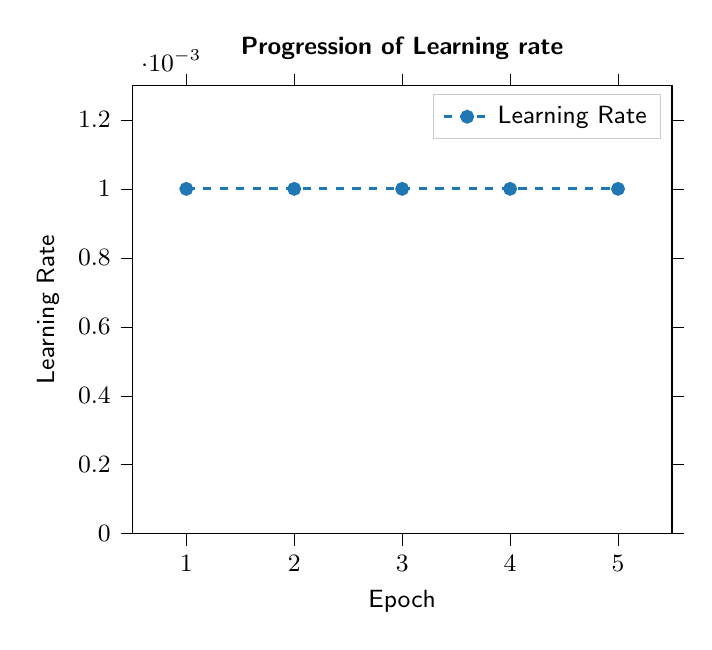
\begin{tikzpicture}

\definecolor{color0}{rgb}{0.12156862745098,0.466666666666667,0.705882352941177}

\begin{axis}[
font=\small,
legend cell align={left},
legend style={draw=white!80.0!black},
minor xtick={},
minor ytick={},
tick align=outside,
tick pos=both,
title={{\bf Progression of Learning rate}},
x grid style={white!69.01960784313725!black},
xlabel={Epoch},
xmin=0.5, xmax=5.5,
xtick style={color=black},
xtick={1,2,3,4,5},
y grid style={white!69.01960784313725!black},
ylabel={Learning Rate},
ymin=0, ymax=0.0013,
ytick style={color=black},
ytick={0,0.0002,0.0004,0.0006,0.0008,0.001,0.0012,0.0014}
]
\addplot [line width=1.0pt, color0, dashed, mark=*, mark size=2, mark options={solid}]
table {%
1 0.001
2 0.001
3 0.001
4 0.001
5 0.001
};
\addlegendentry{Learning Rate}
\end{axis}

\end{tikzpicture}
            \caption{Learning rate per epoch for model \protect\hyperref[training:7]
                        {7}.}
        \end{subfigure}%
        \caption{Training and evaluation metrics for model  \protect\hyperref[training:7]
                    {7}.
                \label{fig:results7}}
    \end{figure}

    \subsubsection*{Dataset}
    \begin{description}
        \item[Name] MNIST
        \item[Train-Test-Dev split:] {\it Training set:}
        60000,
        {\it Test set:}
        10000,
        {\it Dev set:}
        0,
        \item[Image size] [28, 28]


    \end{description}
    %
    \subsubsection*{Training}
    \begin{description}
        \item[Number of epochs] 5
        \item[Optimizer] Adam (Kingma et al., 2015)

            \begin{tabular}{rl}
                    {\bf Learning Rate} & 0.0010000000474974513 \\
                    {\bf Beta 1} & 0.8999999761581421 \\
                    {\bf Beta 2} & 0.9990000128746033 \\
                    {\bf Decay} & 0.0 \\
                    {\bf Epsilon} & 1e-07 \\
                    {\bf Amsgrad} & False \\
            \end{tabular}

        \item[Loss] Categorical crossentropy
        \item[Batch size] 128
        \item[Shuffle] Yes
        \item[Training time] 18 sec
    \end{description}
    %
    \subsubsection*{Platform}
    \begin{description}
        \item[Weights exported to path] weights\textbackslash MLP2layers\_5ep\_MNIST.h5
        \item[Device used] GPU (GeForce GTX 1060 6GB)
        \item[CPU] Intel(R) Xeon(R) CPU E3-1245 v5 @ 3.50GHz,
                   X86\_64
        \item[Python Version] 3.7.2.final.0 (64 bit)
        \item[Keras Version] 2.2.5 (Backend: tensorflow)
        \item[Tensorflow Version] 1.14.0
        \item[Timestamp] 25.09.2019 at 16:05
    \end{description}
    \subsection{Model 8:
                        MLP2layers
                \label{training:8}
                }
    %
    \paragraph*{Training history} See Figure \ref{fig:results8}.
    \begin{figure}[H]
        \centering
        \begin{subfigure}{.5\textwidth}
            % This file was created by tikzplotlib v0.8.2.
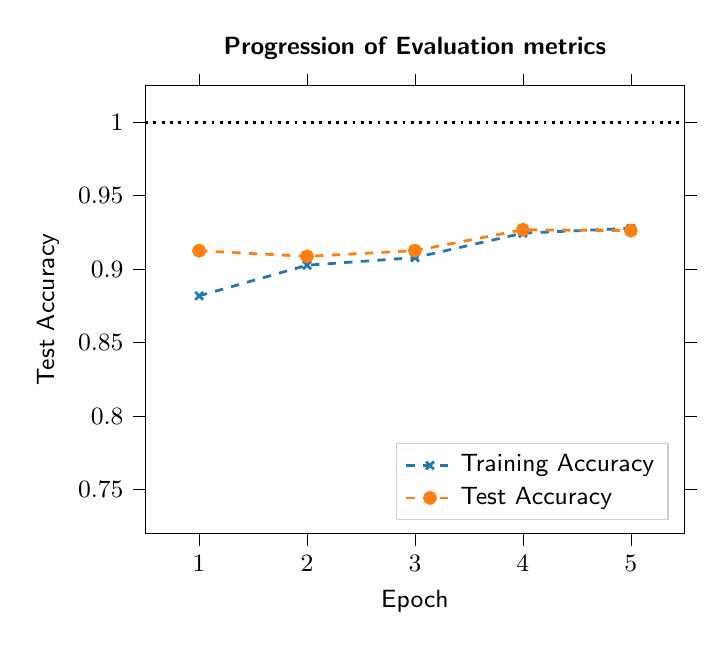
\begin{tikzpicture}

\definecolor{color0}{rgb}{0.12156862745098,0.466666666666667,0.705882352941177}
\definecolor{color1}{rgb}{1,0.498039215686275,0.0549019607843137}

\begin{axis}[
font=\small,
legend cell align={left},
legend style={at={(0.97,0.03)}, anchor=south east, draw=white!80.0!black},
minor xtick={},
minor ytick={},
tick align=outside,
tick pos=both,
title={{\bf Progression of Evaluation metrics}},
x grid style={white!69.01960784313725!black},
xlabel={Epoch},
xmin=0.5, xmax=5.5,
xtick style={color=black},
xtick={1,2,3,4,5},
y grid style={white!69.01960784313725!black},
ylabel={Test Accuracy},
ymin=0.72, ymax=1.025,
ytick style={color=black},
ytick={0.7,0.75,0.8,0.85,0.9,0.95,1,1.05}
]
\addplot [line width=1.0pt, color0, dashed, mark=x, mark size=2, mark options={solid}]
table {%
1 0.881816666698456
2 0.902666666634877
3 0.907849999968211
4 0.924483333301544
5 0.927783333333333
};
\addlegendentry{Training Accuracy}
\addplot [line width=1.0pt, color1, dashed, mark=*, mark size=2, mark options={solid}]
table {%
1 0.9125
2 0.9087
3 0.9126
4 0.9268
5 0.9262
};
\addlegendentry{Test Accuracy}
\addplot [line width=1.0pt, black, dotted, forget plot]
table {%
0.5 1
5.5 1
};
\end{axis}

\end{tikzpicture}
            \caption{Accuracy learning process for model \protect\hyperref[training:8]
                        {8}.}
        \end{subfigure}%
        \hfill%
        \begin{subfigure}{.5\textwidth}
            % This file was created by tikzplotlib v0.8.2.
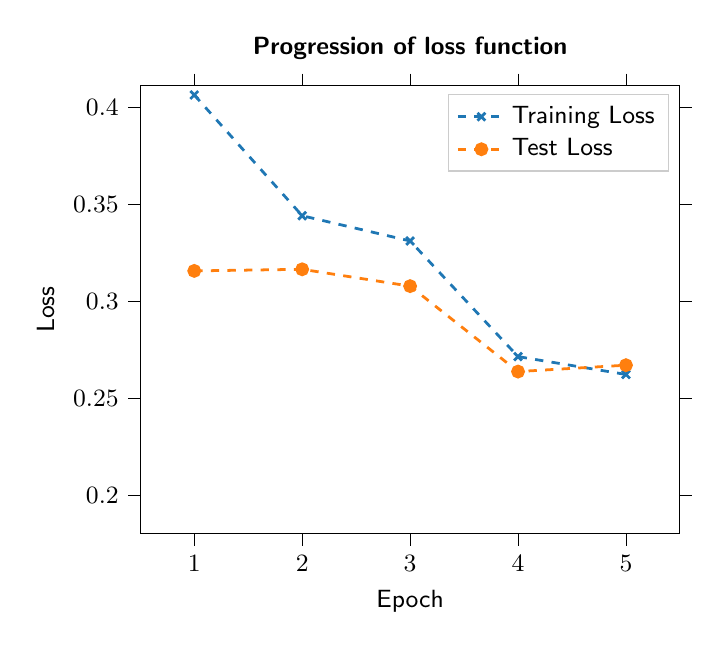
\begin{tikzpicture}

\definecolor{color0}{rgb}{0.12156862745098,0.466666666666667,0.705882352941177}
\definecolor{color1}{rgb}{1,0.498039215686275,0.0549019607843137}

\begin{axis}[
font=\small,
legend cell align={left},
legend style={draw=white!80.0!black},
minor xtick={},
minor ytick={},
tick align=outside,
tick pos=both,
title={{\bf Progression of loss function}},
x grid style={white!69.01960784313725!black},
xlabel={Epoch},
xmin=0.5, xmax=5.5,
xtick style={color=black},
xtick={1,2,3,4,5},
y grid style={white!69.01960784313725!black},
ylabel={Loss},
ymin=0.18, ymax=0.41153484153986,
ytick style={color=black},
ytick={0.15,0.2,0.25,0.3,0.35,0.4,0.45}
]
\addplot [line width=1.0pt, color0, dashed, mark=x, mark size=2, mark options={solid}]
table {%
1 0.406608191045125
2 0.344228831338882
3 0.331202676916122
4 0.271477153873444
5 0.262256178998947
};
\addlegendentry{Training Loss}
\addplot [line width=1.0pt, color1, dashed, mark=*, mark size=2, mark options={solid}]
table {%
1 0.315740000867844
2 0.316565262722969
3 0.307874956035614
4 0.263751934981346
5 0.267048618364334
};
\addlegendentry{Test Loss}
\end{axis}

\end{tikzpicture}
            \caption{Loss learning process for model \protect\hyperref[training:8]
                        {8}.}
        \end{subfigure}
        \par\bigskip
        \begin{subfigure}{.5\textwidth}
            % This file was created by tikzplotlib v0.8.2.
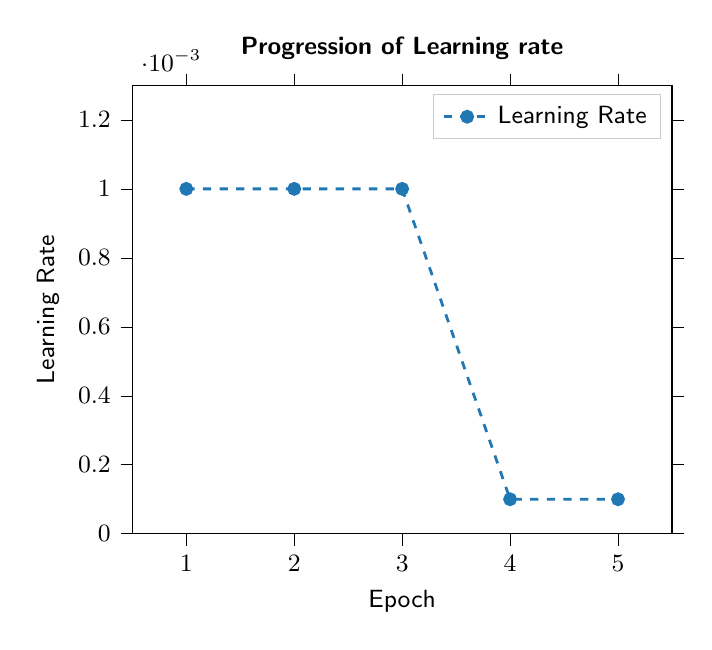
\begin{tikzpicture}

\definecolor{color0}{rgb}{0.12156862745098,0.466666666666667,0.705882352941177}

\begin{axis}[
font=\small,
legend cell align={left},
legend style={draw=white!80.0!black},
minor xtick={},
minor ytick={},
tick align=outside,
tick pos=both,
title={{\bf Progression of Learning rate}},
x grid style={white!69.01960784313725!black},
xlabel={Epoch},
xmin=0.5, xmax=5.5,
xtick style={color=black},
xtick={1,2,3,4,5},
y grid style={white!69.01960784313725!black},
ylabel={Learning Rate},
ymin=0, ymax=0.0013,
ytick style={color=black},
ytick={0,0.0002,0.0004,0.0006,0.0008,0.001,0.0012,0.0014}
]
\addplot [line width=1.0pt, color0, dashed, mark=*, mark size=2, mark options={solid}]
table {%
1 0.001
2 0.001
3 0.001
4 0.000100000005
5 0.000100000005
};
\addlegendentry{Learning Rate}
\end{axis}

\end{tikzpicture}
            \caption{Learning rate per epoch for model \protect\hyperref[training:8]
                        {8}.}
        \end{subfigure}%
        \caption{Training and evaluation metrics for model  \protect\hyperref[training:8]
                    {8}.
                \label{fig:results8}}
    \end{figure}

    \subsubsection*{Dataset}
    \begin{description}
        \item[Name] MNIST
        \item[Train-Test-Dev split:] {\it Training set:}
        60000,
        {\it Test set:}
        10000,
        {\it Dev set:}
        0,
        \item[Image size] [28, 28]


    \end{description}
    %
    \subsubsection*{Training}
    \begin{description}
        \item[Number of epochs] 5
        \item[Optimizer] Adam (Kingma et al., 2015)

            \begin{tabular}{rl}
                    {\bf Learning Rate} & 0.00010000000474974513 \\
                    {\bf Beta 1} & 0.8999999761581421 \\
                    {\bf Beta 2} & 0.9990000128746033 \\
                    {\bf Decay} & 0.0 \\
                    {\bf Epsilon} & 1e-07 \\
                    {\bf Amsgrad} & False \\
            \end{tabular}

        \item[Loss] Categorical crossentropy
        \item[Batch size] 128
        \item[Shuffle] Yes
        \item[Training time] 19 sec
    \end{description}
    %
    \subsubsection*{Platform}
    \begin{description}
        \item[Weights exported to path] weights\textbackslash MLP2layers\_5ep\_MNIST.h5
        \item[Device used] GPU (GeForce GTX 1060 6GB)
        \item[CPU] Intel(R) Xeon(R) CPU E3-1245 v5 @ 3.50GHz,
                   X86\_64
        \item[Python Version] 3.7.2.final.0 (64 bit)
        \item[Keras Version] 2.2.5 (Backend: tensorflow)
        \item[Tensorflow Version] 1.14.0
        \item[Timestamp] 25.09.2019 at 16:08
    \end{description}
    \subsection{Model 9:
                        MLP2layers
                \label{training:9}
                }
    %
    \paragraph*{Training history} See Figure \ref{fig:results9}.
    \begin{figure}[H]
        \centering
        \begin{subfigure}{.5\textwidth}
            % This file was created by tikzplotlib v0.8.2.
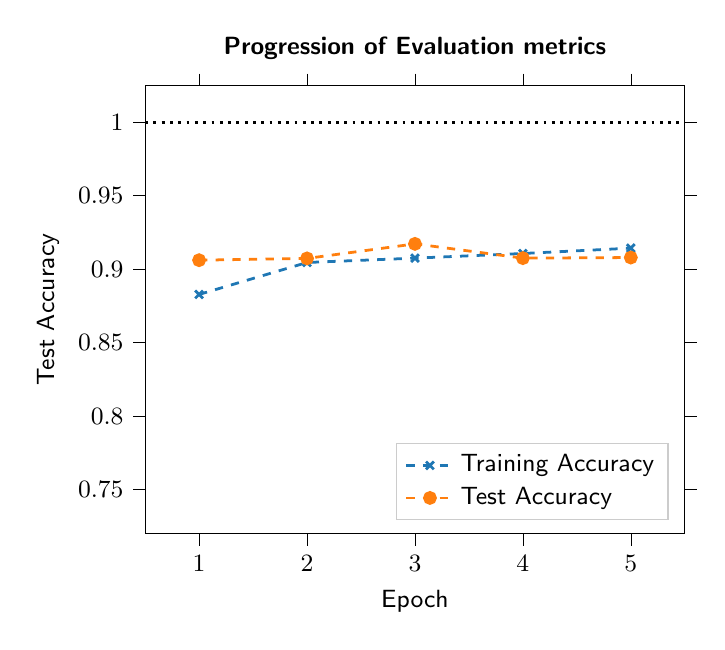
\begin{tikzpicture}

\definecolor{color0}{rgb}{0.12156862745098,0.466666666666667,0.705882352941177}
\definecolor{color1}{rgb}{1,0.498039215686275,0.0549019607843137}

\begin{axis}[
font=\small,
legend cell align={left},
legend style={at={(0.97,0.03)}, anchor=south east, draw=white!80.0!black},
minor xtick={},
minor ytick={},
tick align=outside,
tick pos=both,
title={{\bf Progression of Evaluation metrics}},
x grid style={white!69.01960784313725!black},
xlabel={Epoch},
xmin=0.5, xmax=5.5,
xtick style={color=black},
xtick={1,2,3,4,5},
y grid style={white!69.01960784313725!black},
ylabel={Test Accuracy},
ymin=0.72, ymax=1.025,
ytick style={color=black},
ytick={0.7,0.75,0.8,0.85,0.9,0.95,1,1.05}
]
\addplot [line width=1.0pt, color0, dashed, mark=x, mark size=2, mark options={solid}]
table {%
1 0.8828
2 0.904533333365122
3 0.907499999968211
4 0.910650000031789
5 0.914300000031789
};
\addlegendentry{Training Accuracy}
\addplot [line width=1.0pt, color1, dashed, mark=*, mark size=2, mark options={solid}]
table {%
1 0.9061
2 0.9073
3 0.9172
4 0.9075
5 0.9079
};
\addlegendentry{Test Accuracy}
\addplot [line width=1.0pt, black, dotted, forget plot]
table {%
0.5 1
5.5 1
};
\end{axis}

\end{tikzpicture}
            \caption{Accuracy learning process for model \protect\hyperref[training:9]
                        {9}.}
        \end{subfigure}%
        \hfill%
        \begin{subfigure}{.5\textwidth}
            % This file was created by tikzplotlib v0.8.2.
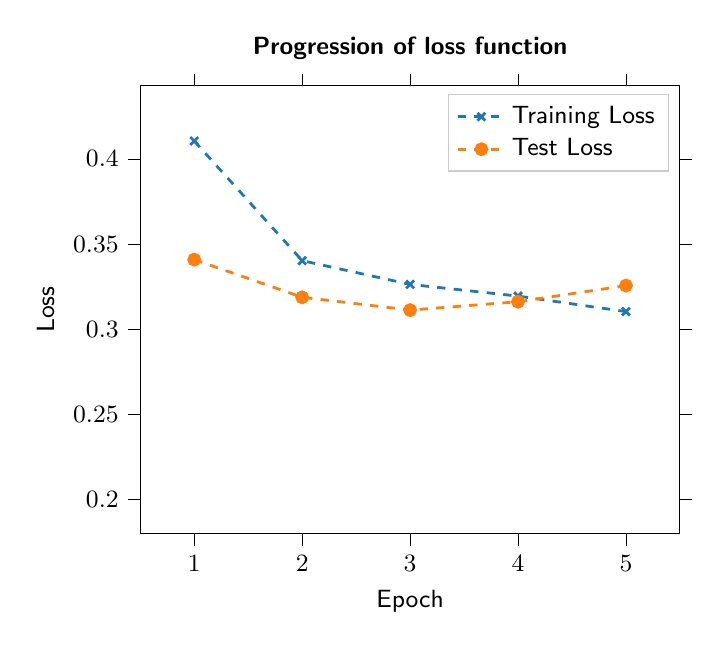
\begin{tikzpicture}

\definecolor{color0}{rgb}{0.12156862745098,0.466666666666667,0.705882352941177}
\definecolor{color1}{rgb}{1,0.498039215686275,0.0549019607843137}

\begin{axis}[
font=\small,
legend cell align={left},
legend style={draw=white!80.0!black},
minor xtick={},
minor ytick={},
tick align=outside,
tick pos=both,
title={{\bf Progression of loss function}},
x grid style={white!69.01960784313725!black},
xlabel={Epoch},
xmin=0.5, xmax=5.5,
xtick style={color=black},
xtick={1,2,3,4,5},
y grid style={white!69.01960784313725!black},
ylabel={Loss},
ymin=0.18, ymax=0.443148319344521,
ytick style={color=black},
ytick={0.15,0.2,0.25,0.3,0.35,0.4,0.45}
]
\addplot [line width=1.0pt, color0, dashed, mark=x, mark size=2, mark options={solid}]
table {%
1 0.410522589842478
2 0.340279855410258
3 0.326354736709595
4 0.319477715015411
5 0.310384571854273
};
\addlegendentry{Training Loss}
\addplot [line width=1.0pt, color1, dashed, mark=*, mark size=2, mark options={solid}]
table {%
1 0.340883322572708
2 0.318791474246979
3 0.311260000741482
4 0.316177561283112
5 0.325653813743591
};
\addlegendentry{Test Loss}
\end{axis}

\end{tikzpicture}
            \caption{Loss learning process for model \protect\hyperref[training:9]
                        {9}.}
        \end{subfigure}
        \par\bigskip
        \begin{subfigure}{.5\textwidth}
            % This file was created by tikzplotlib v0.8.2.
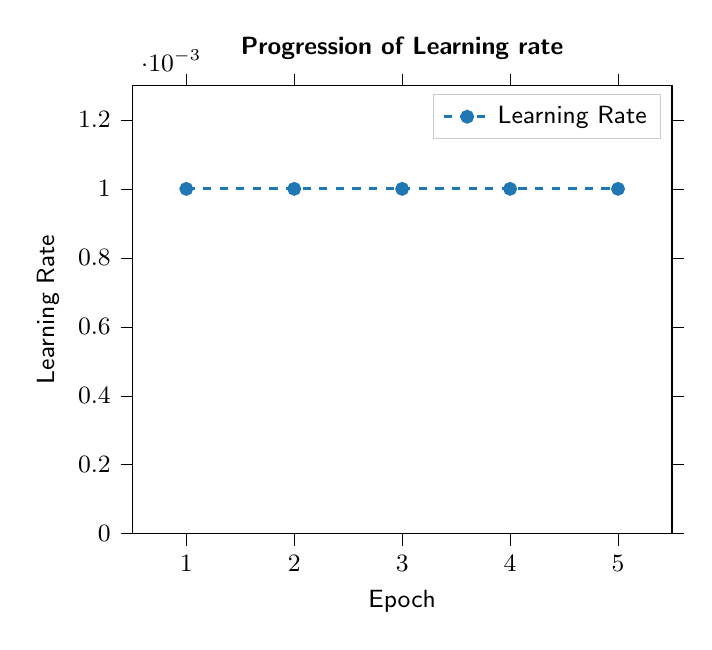
\begin{tikzpicture}

\definecolor{color0}{rgb}{0.12156862745098,0.466666666666667,0.705882352941177}

\begin{axis}[
font=\small,
legend cell align={left},
legend style={draw=white!80.0!black},
minor xtick={},
minor ytick={},
tick align=outside,
tick pos=both,
title={{\bf Progression of Learning rate}},
x grid style={white!69.01960784313725!black},
xlabel={Epoch},
xmin=0.5, xmax=5.5,
xtick style={color=black},
xtick={1,2,3,4,5},
y grid style={white!69.01960784313725!black},
ylabel={Learning Rate},
ymin=0, ymax=0.0013,
ytick style={color=black},
ytick={0,0.0002,0.0004,0.0006,0.0008,0.001,0.0012,0.0014}
]
\addplot [line width=1.0pt, color0, dashed, mark=*, mark size=2, mark options={solid}]
table {%
1 0.001
2 0.001
3 0.001
4 0.001
5 0.001
};
\addlegendentry{Learning Rate}
\end{axis}

\end{tikzpicture}
            \caption{Learning rate per epoch for model \protect\hyperref[training:9]
                        {9}.}
        \end{subfigure}%
        \caption{Training and evaluation metrics for model  \protect\hyperref[training:9]
                    {9}.
                \label{fig:results9}}
    \end{figure}

    \subsubsection*{Dataset}
    \begin{description}
        \item[Name] MNIST
        \item[Train-Test-Dev split:] {\it Training set:}
        60000,
        {\it Test set:}
        10000,
        {\it Dev set:}
        0,
        \item[Image size] [28, 28]


    \end{description}
    %
    \subsubsection*{Training}
    \begin{description}
        \item[Number of epochs] 5
        \item[Optimizer] Adam (Kingma et al., 2015)

            \begin{tabular}{rl}
                    {\bf Learning Rate} & 0.00010000000474974513 \\
                    {\bf Beta 1} & 0.8999999761581421 \\
                    {\bf Beta 2} & 0.9990000128746033 \\
                    {\bf Decay} & 0.0 \\
                    {\bf Epsilon} & 1e-07 \\
                    {\bf Amsgrad} & False \\
            \end{tabular}

        \item[Loss] Categorical crossentropy
        \item[Batch size] 128
        \item[Shuffle] Yes
        \item[Training time] 18 sec
    \end{description}
    %
    \subsubsection*{Platform}
    \begin{description}
        \item[Weights exported to path] weights\textbackslash MLP2layers\_5ep\_MNIST.h5
        \item[Device used] GPU (GeForce GTX 1060 6GB)
        \item[CPU] Intel(R) Xeon(R) CPU E3-1245 v5 @ 3.50GHz,
                   X86\_64
        \item[Python Version] 3.7.2.final.0 (64 bit)
        \item[Keras Version] 2.2.5 (Backend: tensorflow)
        \item[Tensorflow Version] 1.14.0
        \item[Timestamp] 25.09.2019 at 16:10
    \end{description}
    \subsection{Model 10:
                        MLP5layers
                \label{training:10}
                }
    %
    \paragraph*{Training history} See Figure \ref{fig:results10}.
    \begin{figure}[H]
        \centering
        \begin{subfigure}{.5\textwidth}
            % This file was created by tikzplotlib v0.8.2.
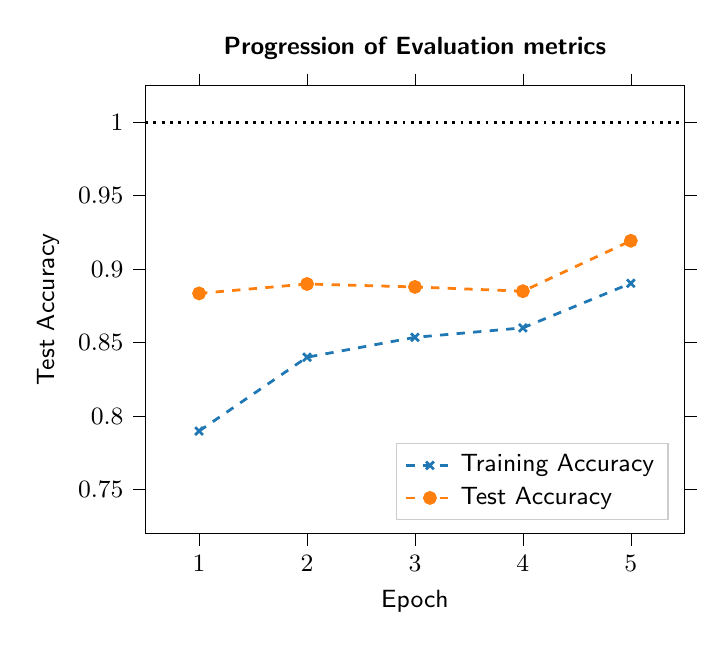
\begin{tikzpicture}

\definecolor{color0}{rgb}{0.12156862745098,0.466666666666667,0.705882352941177}
\definecolor{color1}{rgb}{1,0.498039215686275,0.0549019607843137}

\begin{axis}[
font=\small,
legend cell align={left},
legend style={at={(0.97,0.03)}, anchor=south east, draw=white!80.0!black},
minor xtick={},
minor ytick={},
tick align=outside,
tick pos=both,
title={{\bf Progression of Evaluation metrics}},
x grid style={white!69.01960784313725!black},
xlabel={Epoch},
xmin=0.5, xmax=5.5,
xtick style={color=black},
xtick={1,2,3,4,5},
y grid style={white!69.01960784313725!black},
ylabel={Test Accuracy},
ymin=0.72, ymax=1.025,
ytick style={color=black},
ytick={0.7,0.75,0.8,0.85,0.9,0.95,1,1.05}
]
\addplot [line width=1.0pt, color0, dashed, mark=x, mark size=2, mark options={solid}]
table {%
1 0.789849999968211
2 0.840083333333333
3 0.853616666666667
4 0.860066666698456
5 0.890366666666667
};
\addlegendentry{Training Accuracy}
\addplot [line width=1.0pt, color1, dashed, mark=*, mark size=2, mark options={solid}]
table {%
1 0.8835
2 0.8899
3 0.8879
4 0.885
5 0.9193
};
\addlegendentry{Test Accuracy}
\addplot [line width=1.0pt, black, dotted, forget plot]
table {%
0.5 1
5.5 1
};
\end{axis}

\end{tikzpicture}
            \caption{Accuracy learning process for model \protect\hyperref[training:10]
                        {10}.}
        \end{subfigure}%
        \hfill%
        \begin{subfigure}{.5\textwidth}
            % This file was created by tikzplotlib v0.8.2.
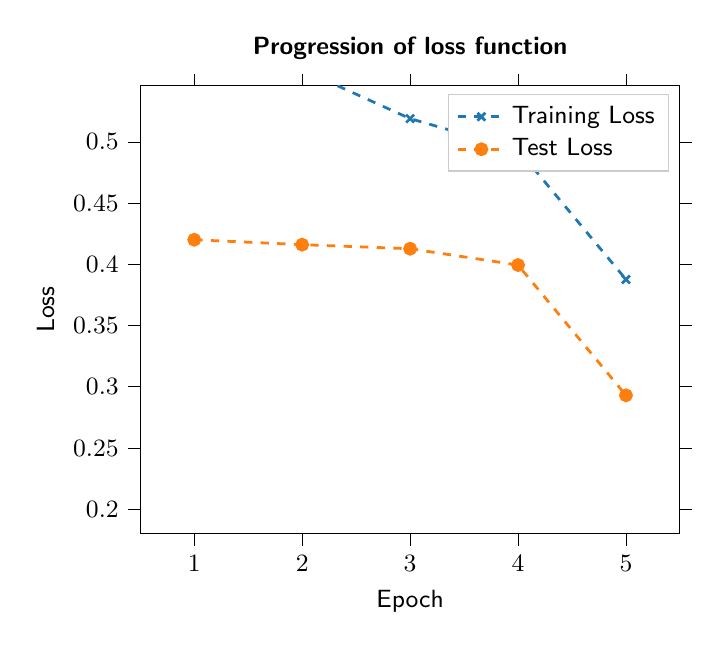
\begin{tikzpicture}

\definecolor{color0}{rgb}{0.12156862745098,0.466666666666667,0.705882352941177}
\definecolor{color1}{rgb}{1,0.498039215686275,0.0549019607843137}

\begin{axis}[
font=\small,
legend cell align={left},
legend style={draw=white!80.0!black},
minor xtick={},
minor ytick={},
tick align=outside,
tick pos=both,
title={{\bf Progression of loss function}},
x grid style={white!69.01960784313725!black},
xlabel={Epoch},
xmin=0.5, xmax=5.5,
xtick style={color=black},
xtick={1,2,3,4,5},
y grid style={white!69.01960784313725!black},
ylabel={Loss},
ymin=0.18, ymax=0.546048210976124,
ytick style={color=black},
ytick={0.15,0.2,0.25,0.3,0.35,0.4,0.45,0.5,0.55}
]
\addplot [line width=1.0pt, color0, dashed, mark=x, mark size=2, mark options={solid}]
table {%
1 0.721805390199025
2 0.558844729804993
3 0.518933760706584
4 0.493574853467941
5 0.38762162211736
};
\addlegendentry{Training Loss}
\addplot [line width=1.0pt, color1, dashed, mark=*, mark size=2, mark options={solid}]
table {%
1 0.420037085366249
2 0.416019944572449
3 0.412705702161789
4 0.399392964076996
5 0.293000747227669
};
\addlegendentry{Test Loss}
\end{axis}

\end{tikzpicture}
            \caption{Loss learning process for model \protect\hyperref[training:10]
                        {10}.}
        \end{subfigure}
        \par\bigskip
        \begin{subfigure}{.5\textwidth}
            % This file was created by tikzplotlib v0.8.2.
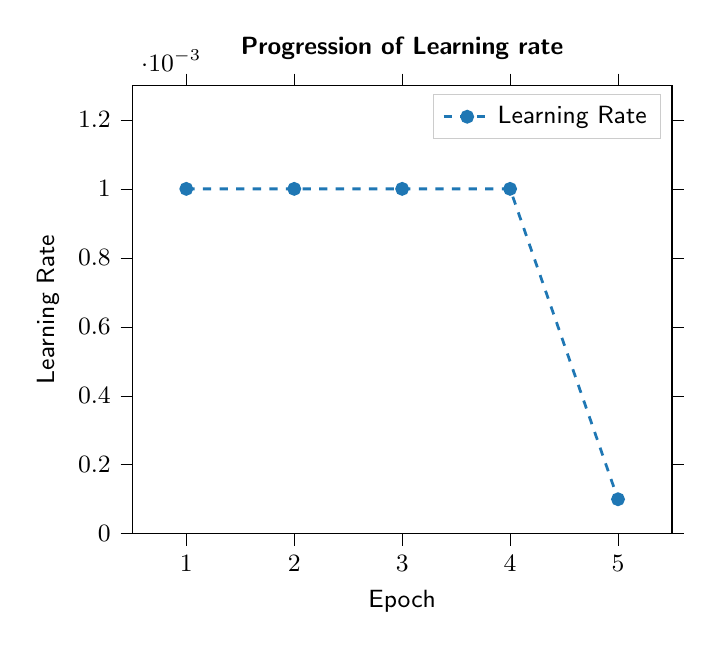
\begin{tikzpicture}

\definecolor{color0}{rgb}{0.12156862745098,0.466666666666667,0.705882352941177}

\begin{axis}[
font=\small,
legend cell align={left},
legend style={draw=white!80.0!black},
minor xtick={},
minor ytick={},
tick align=outside,
tick pos=both,
title={{\bf Progression of Learning rate}},
x grid style={white!69.01960784313725!black},
xlabel={Epoch},
xmin=0.5, xmax=5.5,
xtick style={color=black},
xtick={1,2,3,4,5},
y grid style={white!69.01960784313725!black},
ylabel={Learning Rate},
ymin=0, ymax=0.0013,
ytick style={color=black},
ytick={0,0.0002,0.0004,0.0006,0.0008,0.001,0.0012,0.0014}
]
\addplot [line width=1.0pt, color0, dashed, mark=*, mark size=2, mark options={solid}]
table {%
1 0.001
2 0.001
3 0.001
4 0.001
5 0.000100000005
};
\addlegendentry{Learning Rate}
\end{axis}

\end{tikzpicture}
            \caption{Learning rate per epoch for model \protect\hyperref[training:10]
                        {10}.}
        \end{subfigure}%
        \caption{Training and evaluation metrics for model  \protect\hyperref[training:10]
                    {10}.
                \label{fig:results10}}
    \end{figure}

    \subsubsection*{Dataset}
    \begin{description}
        \item[Name] MNIST
        \item[Train-Test-Dev split:] {\it Training set:}
        60000,
        {\it Test set:}
        10000,
        {\it Dev set:}
        0,
        \item[Image size] [28, 28]


    \end{description}
    %
    \subsubsection*{Training}
    \begin{description}
        \item[Number of epochs] 5
        \item[Optimizer] RMSProp 

            \begin{tabular}{rl}
                    {\bf Learning Rate} & 0.00010000000474974513 \\
                    {\bf Rho} & 0.8999999761581421 \\
                    {\bf Decay} & 0.0 \\
                    {\bf Epsilon} & 1e-07 \\
            \end{tabular}

        \item[Loss] Categorical crossentropy
        \item[Batch size] 128
        \item[Shuffle] Yes
        \item[Training time] 23 sec
    \end{description}
    %
    \subsubsection*{Platform}
    \begin{description}
        \item[Weights exported to path] weights\textbackslash MLP5layers\_5ep\_MNIST.h5
        \item[Device used] GPU (GeForce GTX 1060 6GB)
        \item[CPU] Intel(R) Xeon(R) CPU E3-1245 v5 @ 3.50GHz,
                   X86\_64
        \item[Python Version] 3.7.2.final.0 (64 bit)
        \item[Keras Version] 2.2.5 (Backend: tensorflow)
        \item[Tensorflow Version] 1.14.0
        \item[Timestamp] 25.09.2019 at 16:08
    \end{description}
    \subsection{Model 11:
                        MLP5layers
                \label{training:11}
                }
    %
    \paragraph*{Training history} See Figure \ref{fig:results11}.
    \begin{figure}[H]
        \centering
        \begin{subfigure}{.5\textwidth}
            % This file was created by tikzplotlib v0.8.2.
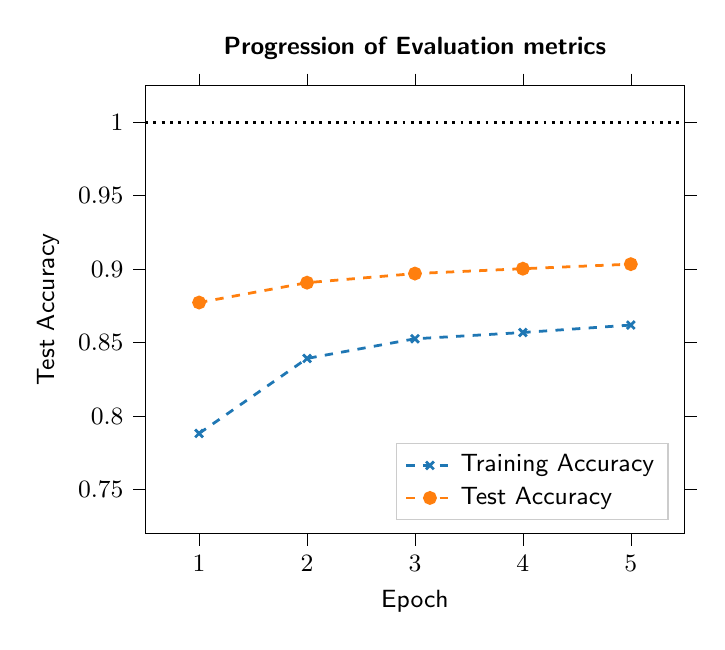
\begin{tikzpicture}

\definecolor{color0}{rgb}{0.12156862745098,0.466666666666667,0.705882352941177}
\definecolor{color1}{rgb}{1,0.498039215686275,0.0549019607843137}

\begin{axis}[
font=\small,
legend cell align={left},
legend style={at={(0.97,0.03)}, anchor=south east, draw=white!80.0!black},
minor xtick={},
minor ytick={},
tick align=outside,
tick pos=both,
title={{\bf Progression of Evaluation metrics}},
x grid style={white!69.01960784313725!black},
xlabel={Epoch},
xmin=0.5, xmax=5.5,
xtick style={color=black},
xtick={1,2,3,4,5},
y grid style={white!69.01960784313725!black},
ylabel={Test Accuracy},
ymin=0.72, ymax=1.025,
ytick style={color=black},
ytick={0.7,0.75,0.8,0.85,0.9,0.95,1,1.05}
]
\addplot [line width=1.0pt, color0, dashed, mark=x, mark size=2, mark options={solid}]
table {%
1 0.788233333301544
2 0.83925
3 0.852633333301544
4 0.8569
5 0.861966666666667
};
\addlegendentry{Training Accuracy}
\addplot [line width=1.0pt, color1, dashed, mark=*, mark size=2, mark options={solid}]
table {%
1 0.8773
2 0.8908
3 0.897
4 0.9003
5 0.9034
};
\addlegendentry{Test Accuracy}
\addplot [line width=1.0pt, black, dotted, forget plot]
table {%
0.5 1
5.5 1
};
\end{axis}

\end{tikzpicture}
            \caption{Accuracy learning process for model \protect\hyperref[training:11]
                        {11}.}
        \end{subfigure}%
        \hfill%
        \begin{subfigure}{.5\textwidth}
            % This file was created by tikzplotlib v0.8.2.
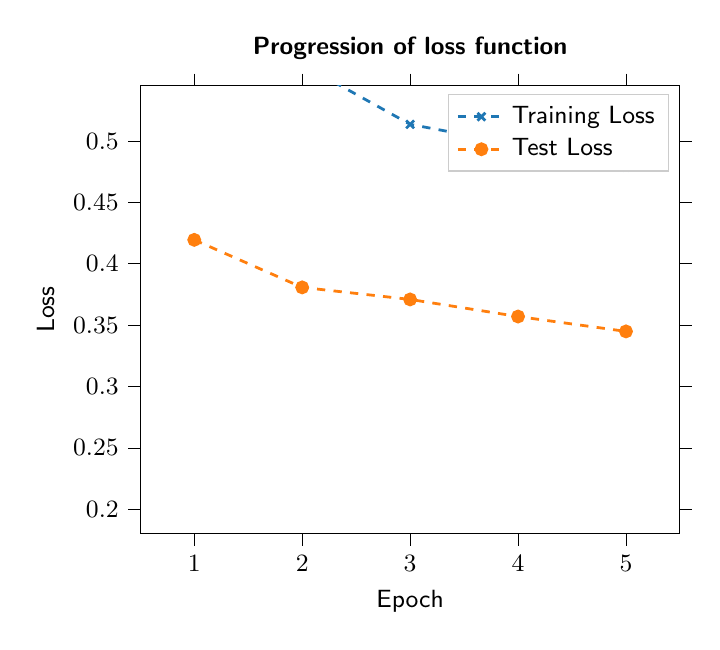
\begin{tikzpicture}

\definecolor{color0}{rgb}{0.12156862745098,0.466666666666667,0.705882352941177}
\definecolor{color1}{rgb}{1,0.498039215686275,0.0549019607843137}

\begin{axis}[
font=\small,
legend cell align={left},
legend style={draw=white!80.0!black},
minor xtick={},
minor ytick={},
tick align=outside,
tick pos=both,
title={{\bf Progression of loss function}},
x grid style={white!69.01960784313725!black},
xlabel={Epoch},
xmin=0.5, xmax=5.5,
xtick style={color=black},
xtick={1,2,3,4,5},
y grid style={white!69.01960784313725!black},
ylabel={Loss},
ymin=0.18, ymax=0.545310750718117,
ytick style={color=black},
ytick={0.15,0.2,0.25,0.3,0.35,0.4,0.45,0.5,0.55}
]
\addplot [line width=1.0pt, color0, dashed, mark=x, mark size=2, mark options={solid}]
table {%
1 0.727507707500458
2 0.562469846185048
3 0.513592550460498
4 0.497046242221196
5 0.478739988231659
};
\addlegendentry{Training Loss}
\addplot [line width=1.0pt, color1, dashed, mark=*, mark size=2, mark options={solid}]
table {%
1 0.419469808244705
2 0.380733536076546
3 0.370916838479042
4 0.356998644137383
5 0.34486786839962
};
\addlegendentry{Test Loss}
\end{axis}

\end{tikzpicture}
            \caption{Loss learning process for model \protect\hyperref[training:11]
                        {11}.}
        \end{subfigure}
        \par\bigskip
        \begin{subfigure}{.5\textwidth}
            % This file was created by tikzplotlib v0.8.2.
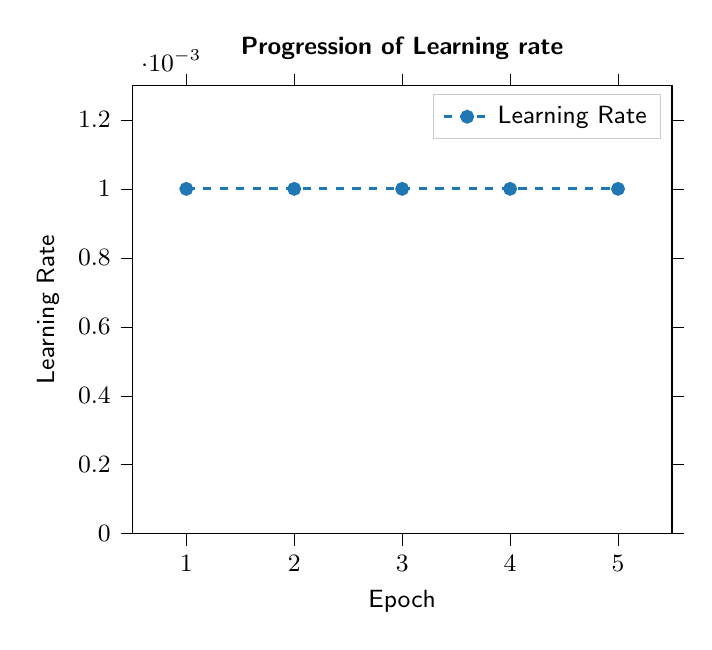
\begin{tikzpicture}

\definecolor{color0}{rgb}{0.12156862745098,0.466666666666667,0.705882352941177}

\begin{axis}[
font=\small,
legend cell align={left},
legend style={draw=white!80.0!black},
minor xtick={},
minor ytick={},
tick align=outside,
tick pos=both,
title={{\bf Progression of Learning rate}},
x grid style={white!69.01960784313725!black},
xlabel={Epoch},
xmin=0.5, xmax=5.5,
xtick style={color=black},
xtick={1,2,3,4,5},
y grid style={white!69.01960784313725!black},
ylabel={Learning Rate},
ymin=0, ymax=0.0013,
ytick style={color=black},
ytick={0,0.0002,0.0004,0.0006,0.0008,0.001,0.0012,0.0014}
]
\addplot [line width=1.0pt, color0, dashed, mark=*, mark size=2, mark options={solid}]
table {%
1 0.001
2 0.001
3 0.001
4 0.001
5 0.001
};
\addlegendentry{Learning Rate}
\end{axis}

\end{tikzpicture}
            \caption{Learning rate per epoch for model \protect\hyperref[training:11]
                        {11}.}
        \end{subfigure}%
        \caption{Training and evaluation metrics for model  \protect\hyperref[training:11]
                    {11}.
                \label{fig:results11}}
    \end{figure}

    \subsubsection*{Dataset}
    \begin{description}
        \item[Name] MNIST
        \item[Train-Test-Dev split:] {\it Training set:}
        60000,
        {\it Test set:}
        10000,
        {\it Dev set:}
        0,
        \item[Image size] [28, 28]


    \end{description}
    %
    \subsubsection*{Training}
    \begin{description}
        \item[Number of epochs] 5
        \item[Optimizer] RMSProp 

            \begin{tabular}{rl}
                    {\bf Learning Rate} & 0.0010000000474974513 \\
                    {\bf Rho} & 0.8999999761581421 \\
                    {\bf Decay} & 0.0 \\
                    {\bf Epsilon} & 1e-07 \\
            \end{tabular}

        \item[Loss] Categorical crossentropy
        \item[Batch size] 128
        \item[Shuffle] Yes
        \item[Training time] 21 sec
    \end{description}
    %
    \subsubsection*{Platform}
    \begin{description}
        \item[Weights exported to path] weights\textbackslash MLP5layers\_5ep\_MNIST.h5
        \item[Device used] GPU (GeForce GTX 1060 6GB)
        \item[CPU] Intel(R) Xeon(R) CPU E3-1245 v5 @ 3.50GHz,
                   X86\_64
        \item[Python Version] 3.7.2.final.0 (64 bit)
        \item[Keras Version] 2.2.5 (Backend: tensorflow)
        \item[Tensorflow Version] 1.14.0
        \item[Timestamp] 25.09.2019 at 16:11
    \end{description}
% %%%%%%%%%%%%%%%%%%%%%%%%%%%%%%%%%%%%%%%%%%%%%%%%%%%%%%%%%%%%%%%%%%%
\newpage
% %%%%%%%%%%%%%%%%%%%%%%%%%%%%%%%%%%%%%%%%%%%%%%%%%%%%%%%%%%%%%%%%%%%
\section{Model Architectures}
\subsection{MLP2layers
            \label{model:MLP2layers}
            }
\paragraph{Used in \No{}:}
    \hyperref[training:5]
             {5},
    \hyperref[training:6]
             {6},
    \hyperref[training:7]
             {7},
    \hyperref[training:8]
             {8},
    \hyperref[training:11]
             {11}
\vspace{-2ex}
%
\paragraph{Model summary:}$\,$\\
\begin{longtable}{rR{.22\textwidth}cL{.22\textwidth}rL{.22\textwidth}}
    \hline\\[-1.5ex]
    \No{} &
    Layer (Type) &
    Output shape &
    Config &
    \#Parameters &
    Inbound layers\\
    \hline\\
    \endhead
        0
        &
        \color{InputLayer}{
        input\_1}
        \color{InputLayer}{
        (InputLayer)}
        &
        (28, 28, 1)
        &
        &
        \num{0}
        &
        \\
        \hline\\[-1.5ex]
        1
        &
        \color{Flatten}{
        flatten\_1}
        \color{Flatten}{
        (Flatten)}
        &
        (784,)
        &
            Parameters of layers of type Flatten not implemented.
        &
        \num{0}
        &
        \color{InputLayer}{
            input\_1}
        \\
        \hline\\[-1.5ex]
        2
        &
        \color{Dense}{
        dense\_1}
        \color{Dense}{
        (Dense)}
        &
        (512,)
        &
            Parameters of layers of type Dense not implemented.
        &
        \num{401920}
        &
        \color{Flatten}{
            flatten\_1}
        \\
        \hline\\[-1.5ex]
        3
        &
        \color{Dropout}{
        dropout\_1}
        \color{Dropout}{
        (Dropout)}
        &
        (512,)
        &
            Parameters of layers of type Dropout not implemented.
        &
        \num{0}
        &
        \color{Dense}{
            dense\_1}
        \\
        \hline\\[-1.5ex]
        4
        &
        \color{Dense}{
        dense\_2}
        \color{Dense}{
        (Dense)}
        &
        (512,)
        &
            Parameters of layers of type Dense not implemented.
        &
        \num{262656}
        &
        \color{Dropout}{
            dropout\_1}
        \\
        \hline\\[-1.5ex]
        5
        &
        \color{Dropout}{
        dropout\_2}
        \color{Dropout}{
        (Dropout)}
        &
        (512,)
        &
            Parameters of layers of type Dropout not implemented.
        &
        \num{0}
        &
        \color{Dense}{
            dense\_2}
        \\
        \hline\\[-1.5ex]
        6
        &
        \color{Dense}{
        dense\_3}
        \color{Dense}{
        (Dense)}
        &
        (10,)
        &
            Parameters of layers of type Dense not implemented.
        &
        \num{5130}
        &
        \color{Dropout}{
            dropout\_2}
        \\
        \hline\\[-1.5ex]
\end{longtable}
\newpage
\subsection{MLP5layers
            \label{model:MLP5layers}
            }
\paragraph{Used in \No{}:}
    \hyperref[training:10]
             {10},
    \hyperref[training:11]
             {11}
\vspace{-2ex}
%
\paragraph{Model summary:}$\,$\\
\begin{longtable}{rR{.22\textwidth}cL{.22\textwidth}rL{.22\textwidth}}
    \hline\\[-1.5ex]
    \No{} &
    Layer (Type) &
    Output shape &
    Config &
    \#Parameters &
    Inbound layers\\
    \hline\\
    \endhead
        0
        &
        \color{InputLayer}{
        input\_5}
        \color{InputLayer}{
        (InputLayer)}
        &
        (28, 28, 1)
        &
        &
        \num{0}
        &
        \\
        \hline\\[-1.5ex]
        1
        &
        \color{Flatten}{
        flatten\_5}
        \color{Flatten}{
        (Flatten)}
        &
        (784,)
        &
            Parameters of layers of type Flatten not implemented.
        &
        \num{0}
        &
        \color{InputLayer}{
            input\_5}
        \\
        \hline\\[-1.5ex]
        2
        &
        \color{Dense}{
        dense\_11}
        \color{Dense}{
        (Dense)}
        &
        (128,)
        &
            Parameters of layers of type Dense not implemented.
        &
        \num{100480}
        &
        \color{Flatten}{
            flatten\_5}
        \\
        \hline\\[-1.5ex]
        3
        &
        \color{Dropout}{
        dropout\_9}
        \color{Dropout}{
        (Dropout)}
        &
        (128,)
        &
            Parameters of layers of type Dropout not implemented.
        &
        \num{0}
        &
        \color{Dense}{
            dense\_11}
        \\
        \hline\\[-1.5ex]
        4
        &
        \color{Dense}{
        dense\_12}
        \color{Dense}{
        (Dense)}
        &
        (256,)
        &
            Parameters of layers of type Dense not implemented.
        &
        \num{33024}
        &
        \color{Dropout}{
            dropout\_9}
        \\
        \hline\\[-1.5ex]
        5
        &
        \color{Dropout}{
        dropout\_10}
        \color{Dropout}{
        (Dropout)}
        &
        (256,)
        &
            Parameters of layers of type Dropout not implemented.
        &
        \num{0}
        &
        \color{Dense}{
            dense\_12}
        \\
        \hline\\[-1.5ex]
        6
        &
        \color{Dense}{
        dense\_13}
        \color{Dense}{
        (Dense)}
        &
        (512,)
        &
            Parameters of layers of type Dense not implemented.
        &
        \num{131584}
        &
        \color{Dropout}{
            dropout\_10}
        \\
        \hline\\[-1.5ex]
        7
        &
        \color{Dropout}{
        dropout\_11}
        \color{Dropout}{
        (Dropout)}
        &
        (512,)
        &
            Parameters of layers of type Dropout not implemented.
        &
        \num{0}
        &
        \color{Dense}{
            dense\_13}
        \\
        \hline\\[-1.5ex]
        8
        &
        \color{Dense}{
        dense\_14}
        \color{Dense}{
        (Dense)}
        &
        (256,)
        &
            Parameters of layers of type Dense not implemented.
        &
        \num{131328}
        &
        \color{Dropout}{
            dropout\_11}
        \\
        \hline\\[-1.5ex]
        9
        &
        \color{Dropout}{
        dropout\_12}
        \color{Dropout}{
        (Dropout)}
        &
        (256,)
        &
            Parameters of layers of type Dropout not implemented.
        &
        \num{0}
        &
        \color{Dense}{
            dense\_14}
        \\
        \hline\\[-1.5ex]
        10
        &
        \color{Dense}{
        dense\_15}
        \color{Dense}{
        (Dense)}
        &
        (128,)
        &
            Parameters of layers of type Dense not implemented.
        &
        \num{32896}
        &
        \color{Dropout}{
            dropout\_12}
        \\
        \hline\\[-1.5ex]
        11
        &
        \color{Dropout}{
        dropout\_13}
        \color{Dropout}{
        (Dropout)}
        &
        (128,)
        &
            Parameters of layers of type Dropout not implemented.
        &
        \num{0}
        &
        \color{Dense}{
            dense\_15}
        \\
        \hline\\[-1.5ex]
        12
        &
        \color{Dense}{
        dense\_16}
        \color{Dense}{
        (Dense)}
        &
        (10,)
        &
            Parameters of layers of type Dense not implemented.
        &
        \num{1290}
        &
        \color{Dropout}{
            dropout\_13}
        \\
        \hline\\[-1.5ex]
\end{longtable}
\newpage
\subsection{ConvNet2layers
            \label{model:ConvNet2layers}
            }
\paragraph{Used in \No{}:}
    \hyperref[training:1]
             {1},
    \hyperref[training:2]
             {2},
    \hyperref[training:3]
             {3},
    \hyperref[training:11]
             {11}
\vspace{-2ex}
%
\paragraph{Model summary:}$\,$\\
\begin{longtable}{rR{.22\textwidth}cL{.22\textwidth}rL{.22\textwidth}}
    \hline\\[-1.5ex]
    \No{} &
    Layer (Type) &
    Output shape &
    Config &
    \#Parameters &
    Inbound layers\\
    \hline\\
    \endhead
        0
        &
        \color{InputLayer}{
        input\_4}
        \color{InputLayer}{
        (InputLayer)}
        &
        (28, 28, 1)
        &
        &
        \num{0}
        &
        \\
        \hline\\[-1.5ex]
        1
        &
        \color{Conv2D}{
        conv2d\_7}
        \color{Conv2D}{
        (Conv2D)}
        &
        (26, 26, 32)
        &
            {\bf Activation:} relu \newline
            {\bf Kernel Size:} [3, 3] \newline
            {\bf Stride:} [1, 1] \newline
            {\bf Dilation:} [1, 1] \newline
            {\bf Padding:} valid
        &
        \num{320}
        &
        \color{InputLayer}{
            input\_4}
        \\
        \hline\\[-1.5ex]
        2
        &
        \color{Conv2D}{
        conv2d\_8}
        \color{Conv2D}{
        (Conv2D)}
        &
        (24, 24, 64)
        &
            {\bf Activation:} relu \newline
            {\bf Kernel Size:} [3, 3] \newline
            {\bf Stride:} [1, 1] \newline
            {\bf Dilation:} [1, 1] \newline
            {\bf Padding:} valid
        &
        \num{18496}
        &
        \color{Conv2D}{
            conv2d\_7}
        \\
        \hline\\[-1.5ex]
        3
        &
        \color{MaxPooling2D}{
        max\_pooling2d\_4}
        \color{MaxPooling2D}{
        (MaxPooling2D)}
        &
        (12, 12, 64)
        &
            {\bf Pool size:} [2, 2] \newline
            {\bf Strides:} [2, 2] \newline
            {\bf Padding:} valid
        &
        \num{0}
        &
        \color{Conv2D}{
            conv2d\_8}
        \\
        \hline\\[-1.5ex]
        4
        &
        \color{Dropout}{
        dropout\_7}
        \color{Dropout}{
        (Dropout)}
        &
        (12, 12, 64)
        &
            Parameters of layers of type Dropout not implemented.
        &
        \num{0}
        &
        \color{MaxPooling2D}{
            max\_pooling2d\_4}
        \\
        \hline\\[-1.5ex]
        5
        &
        \color{Flatten}{
        flatten\_4}
        \color{Flatten}{
        (Flatten)}
        &
        (9216,)
        &
            Parameters of layers of type Flatten not implemented.
        &
        \num{0}
        &
        \color{Dropout}{
            dropout\_7}
        \\
        \hline\\[-1.5ex]
        6
        &
        \color{Dense}{
        dense\_7}
        \color{Dense}{
        (Dense)}
        &
        (128,)
        &
            Parameters of layers of type Dense not implemented.
        &
        \num{1179776}
        &
        \color{Flatten}{
            flatten\_4}
        \\
        \hline\\[-1.5ex]
        7
        &
        \color{Dropout}{
        dropout\_8}
        \color{Dropout}{
        (Dropout)}
        &
        (128,)
        &
            Parameters of layers of type Dropout not implemented.
        &
        \num{0}
        &
        \color{Dense}{
            dense\_7}
        \\
        \hline\\[-1.5ex]
        8
        &
        \color{Dense}{
        dense\_8}
        \color{Dense}{
        (Dense)}
        &
        (10,)
        &
            Parameters of layers of type Dense not implemented.
        &
        \num{1290}
        &
        \color{Dropout}{
            dropout\_8}
        \\
        \hline\\[-1.5ex]
\end{longtable}
\newpage
% %%%%%%%%%%%%%%%%%%%%%%%%%%%%%%%%%%%%%%%%%%%%%%%%%%%%%%%%%%%%%%%%%%%

\end{document}